%%
%% This is file `sigconf.tex',
%% generated with the docstrip utility.
%%
%% The original source files were:
%%
%% samples.dtx  (with options: `all,proceedings,sigconf')
%% 
%% IMPORTANT NOTICE:
%% 
%% For the copyright see the source file.
%% 
%% Any modified versions of this file must be renamed
%% with new filenames distinct from sigconf.tex.
%% 
%% For distribution of the original source see the terms
%% for copying and modification in the file samples.dtx.
%% 
%% This generated file may be distributed as long as the
%% original source files, as listed above, are part of the
%% same distribution. (The sources need not necessarily be
%% in the same archive or directory.)
%%
%%
%% Commands for TeXCount
%TC:macro \cite [option:text,text]
%TC:macro \citep [option:text,text]
%TC:macro \citet [option:text,text]
%TC:envir table 0 1
%TC:envir table* 0 1
%TC:envir tabular [ignore] word
%TC:envir displaymath 0 word
%TC:envir math 0 word
%TC:envir comment 0 0
%%
%% The first command in your LaTeX source must be the \documentclass
%% command.
%%
%% For submission and review of your manuscript please change the
%% command to \documentclass[manuscript, screen, review]{acmart}.
%%
%% When submitting camera ready or to TAPS, please change the command
%% to \documentclass[sigconf]{acmart} or whichever template is required
%% for your publication.
%%
%%
% ASIACCS 2027 uses the latest ACM sigconf format and double-blind review.
% Remove the anonymous and review options only when preparing the camera-ready.
\documentclass[sigconf,anonymous]{acmart}
\usepackage{amsmath,amsfonts}
\usepackage{algorithmic}
\usepackage{algorithm}
\usepackage{array}
\usepackage[caption=false,font=normalsize,labelfont=sf,textfont=sf]{subfig}
\usepackage{textcomp}
\usepackage{stfloats}
\usepackage{url}
\usepackage{verbatim}
\usepackage{graphicx}

\usepackage{multirow}
\usepackage{pifont}
\usepackage{placeins}
\usepackage{float}
\usepackage{amsthm}
\renewcommand{\qedsymbol}{}
\theoremstyle{definition}
\newtheorem{definition}{Definition}
\renewcommand{\thedefinition}{\arabic{definition}}
\theoremstyle{definition}
\newtheorem*{correctness}{Correctness of Unsigncrypt}
\theoremstyle{definition}
\newtheorem*{CRSKey}{Correctness of KeyUpdate}
\theoremstyle{definition}
\newtheorem*{verifiablekeys}{Correctness of Join}
\theoremstyle{definition}
\newtheorem*{Order}{Prevention of Submission-Order Manipulation Attacks}
\theoremstyle{definition}
\newtheorem*{dynamicity}{Dynamicity}
\theoremstyle{definition}
\newtheorem{claim}{Claim}
\theoremstyle{definition}
\newtheorem{assumption}{Assumption}
\theoremstyle{definition}
\newtheorem{theorem}{Theorem}
\renewcommand{\thetheorem}{\arabic{theorem}}
\usepackage{booktabs}

\newcommand{\kms}{km\,s$^{-1}$}
\newcommand{\msun}{$M_\odot}
\newcommand{\getsr}{\leftarrow_{\$}}
\newcommand{\sample}{\getsr} 
\hyphenation{op-tical net-works semi-conduc-tor IEEE-Xplore}
\usepackage{orcidlink}
%%
%% \BibTeX command to typeset BibTeX logo in the docs
\AtBeginDocument{%
  \providecommand\BibTeX{{%
    Bib\TeX}}}

%% Rights management information.  This information is sent to you
%% when you complete the rights form.  These commands have SAMPLE
%% values in them; it is your responsibility as an author to replace
%% the commands and values with those provided to you when you
%% complete the rights form.
\setcopyright{rightsretained}
\settopmatter{printacmref=true,printccs=true,printfolios=true}
\copyrightyear{2027}
\acmYear{2027}
\acmDOI{}
%% DOI, ISBN, and the final rights text are assigned after acceptance.
\acmConference[ASIA CCS '27]{Proceedings of the 2027 ACM Asia Conference on
  Computer and Communications Security}{July 12--16, 2027}{Macau, China}
\acmBooktitle{Proceedings of the 2027 ACM Asia Conference on Computer and
  Communications Security (ASIA CCS '27), July 12--16, 2027, Macau, China}
%%
%%  Uncomment \acmBooktitle if the title of the proceedings is different
%%  from ``Proceedings of ...''!
%%
%%\acmBooktitle{Woodstock '18: ACM Symposium on Neural Gaze Detection,
%%  June 03--05, 2018, Woodstock, NY}
\acmISBN{}


%%
%% Submission ID.
%% Use this when submitting an article to a sponsored event. You'll
%% receive a unique submission ID from the organizers
%% of the event, and this ID should be used as the parameter to this command.
%%\acmSubmissionID{123-A56-BU3}

%%
%% For managing citations, it is recommended to use bibliography
%% files in BibTeX format.
%%
%% You can then either use BibTeX with the ACM-Reference-Format style,
%% or BibLaTeX with the acmnumeric or acmauthoryear sytles, that include
%% support for advanced citation of software artefact from the
%% biblatex-software package, also separately available on CTAN.
%%
%% Look at the sample-*-biblatex.tex files for templates showcasing
%% the biblatex styles.
%%
%%
%% The majority of ACM publications use numbered citations and
%% references.  The command \citestyle{authoryear} switches to the
%% "author year" style.
%%
%% If you are preparing content for an event
%% sponsored by ACM SIGGRAPH, you must use the "author year" style of
%% citations and references.
%% Uncommenting
%% the next command will enable that style.
%%\citestyle{acmauthoryear}


%%
%% end of the preamble, start of the body of the document source.
\begin{document}

%%
%% The "title" command has an optional parameter,
%% allowing the author to define a "short title" to be used in page headers.
\title{FS-DBS: Forward-Secure Distributed Broadcast Signcryption for Secure Cloud-to-Edge Data Distribution}

%%
%% The "author" command and its associated commands are used to define
%% the authors and their affiliations.
%% Of note is the shared affiliation of the first two authors, and the
%% "authornote" and "authornotemark" commands
%% used to denote shared contribution to the research.

%%
%% By default, the full list of authors will be used in the page
%% headers. Often, this list is too long, and will overlap
%% other information printed in the page headers. This command allows
%% the author to define a more concise list
%% of authors' names for this purpose.


%%
%% The abstract is a short summary of the work to be presented in the
%% article.
\begin{abstract}
Edge computing supports applications in manufacturing, artificial intelligence, and other domains. Cloud platforms periodically distribute sensitive data to groups of edge nodes. This process requires confidentiality, source authentication, and forward security. Conventional signcryption is mainly designed for one-to-one communication, while group key agreement (GKA) requires interactive group operations. Broadcast encryption (BE) is better suited to one-to-many distribution, but existing BE schemes satisfy only part of these requirements.

To address these limitations, we propose forward-secure distributed broadcast signcryption (FS-DBS) for cloud-to-edge data distribution. We prove selective forward-secure indistinguishability under chosen-ciphertext attacks (FS-IND-CCA) and selective existential unforgeability under chosen-message attacks (EUF-CMA) under the decisional Bilinear Diffie--Hellman Exponent (dBDHE) assumption. We implement FS-DBS over BLS12-381, achieving 1.11 ms for Signcrypt, 4.63 ms for Unsigncrypt, and 13.20 ms for receiver key update at 1,000 receivers. Compared with the five evaluated schemes, FS-DBS reduces online sender latency by 30.2--71.5\%. FS-DBS also provides constant-size ciphertexts and receiver-set-independent online computation for efficient edge data distribution.

\end{abstract}

%%
%% The code below is generated by the tool at http://dl.acm.org/ccs.cfm.
%% Please copy and paste the code instead of the example below.
%%
\ccsdesc[500]{Security and privacy~Public key encryption}
\ccsdesc[300]{Security and privacy~Key management}
\ccsdesc[300]{Computer systems organization~Cloud computing}
\ccsdesc[300]{Computer systems organization~Embedded and cyber-physical systems}


%%
%% Keywords. The author(s) should pick words that accurately describe
%% the work being presented. Separate the keywords with commas.
\keywords{broadcast encryption, distributed cryptography, edge computing,
forward security, signcryption}
%% A "teaser" image appears between the author and affiliation
%% information and the body of the document, and typically spans the
%% page.



%%
%% This command processes the author and affiliation and title
%% information and builds the first part of the formatted document.
\maketitle


\section{Introduction}
	%边缘计算火热，需要数据分发
	The rapid development of edge computing has enabled a wide range of applications, including manufacturing, smart cities, and artificial intelligence~\cite{satyanarayanan2017edge,roman2018edge}. Distributed neural-network deployments place model components across cloud, edge, and end devices~\cite{teerapittayanon2017ddnn,zhou2019edge}. In these applications, cloud platforms periodically distribute software updates, model parameters, configurations, and other data to groups of geographically dispersed edge nodes. Model parameters may encode commercially valuable functionality and are therefore treated as confidential assets~\cite{tramer2016stealing,jagielski2020extraction}. As the number of edge devices continues to grow, such cloud-to-edge distribution increasingly becomes a fundamental operation of edge computing systems. 
	%现状受到威胁，举例最近的事件
	However, distributing sensitive data to a large group of receivers raises several security requirements. The distributed content must remain confidential and must originate from an authenticated sender. Since edge nodes may operate for long periods in exposed environments, compromise of a current secret key should not reveal data distributed in previous periods. These guarantees should be achieved with low communication and computation overhead to support resource-constrained edge deployments.
\begin{figure}[htbp]
	\centering
	\Description{A cloud provider broadcasts protected software, model, and configuration releases to authorized edge nodes over an untrusted network.}
	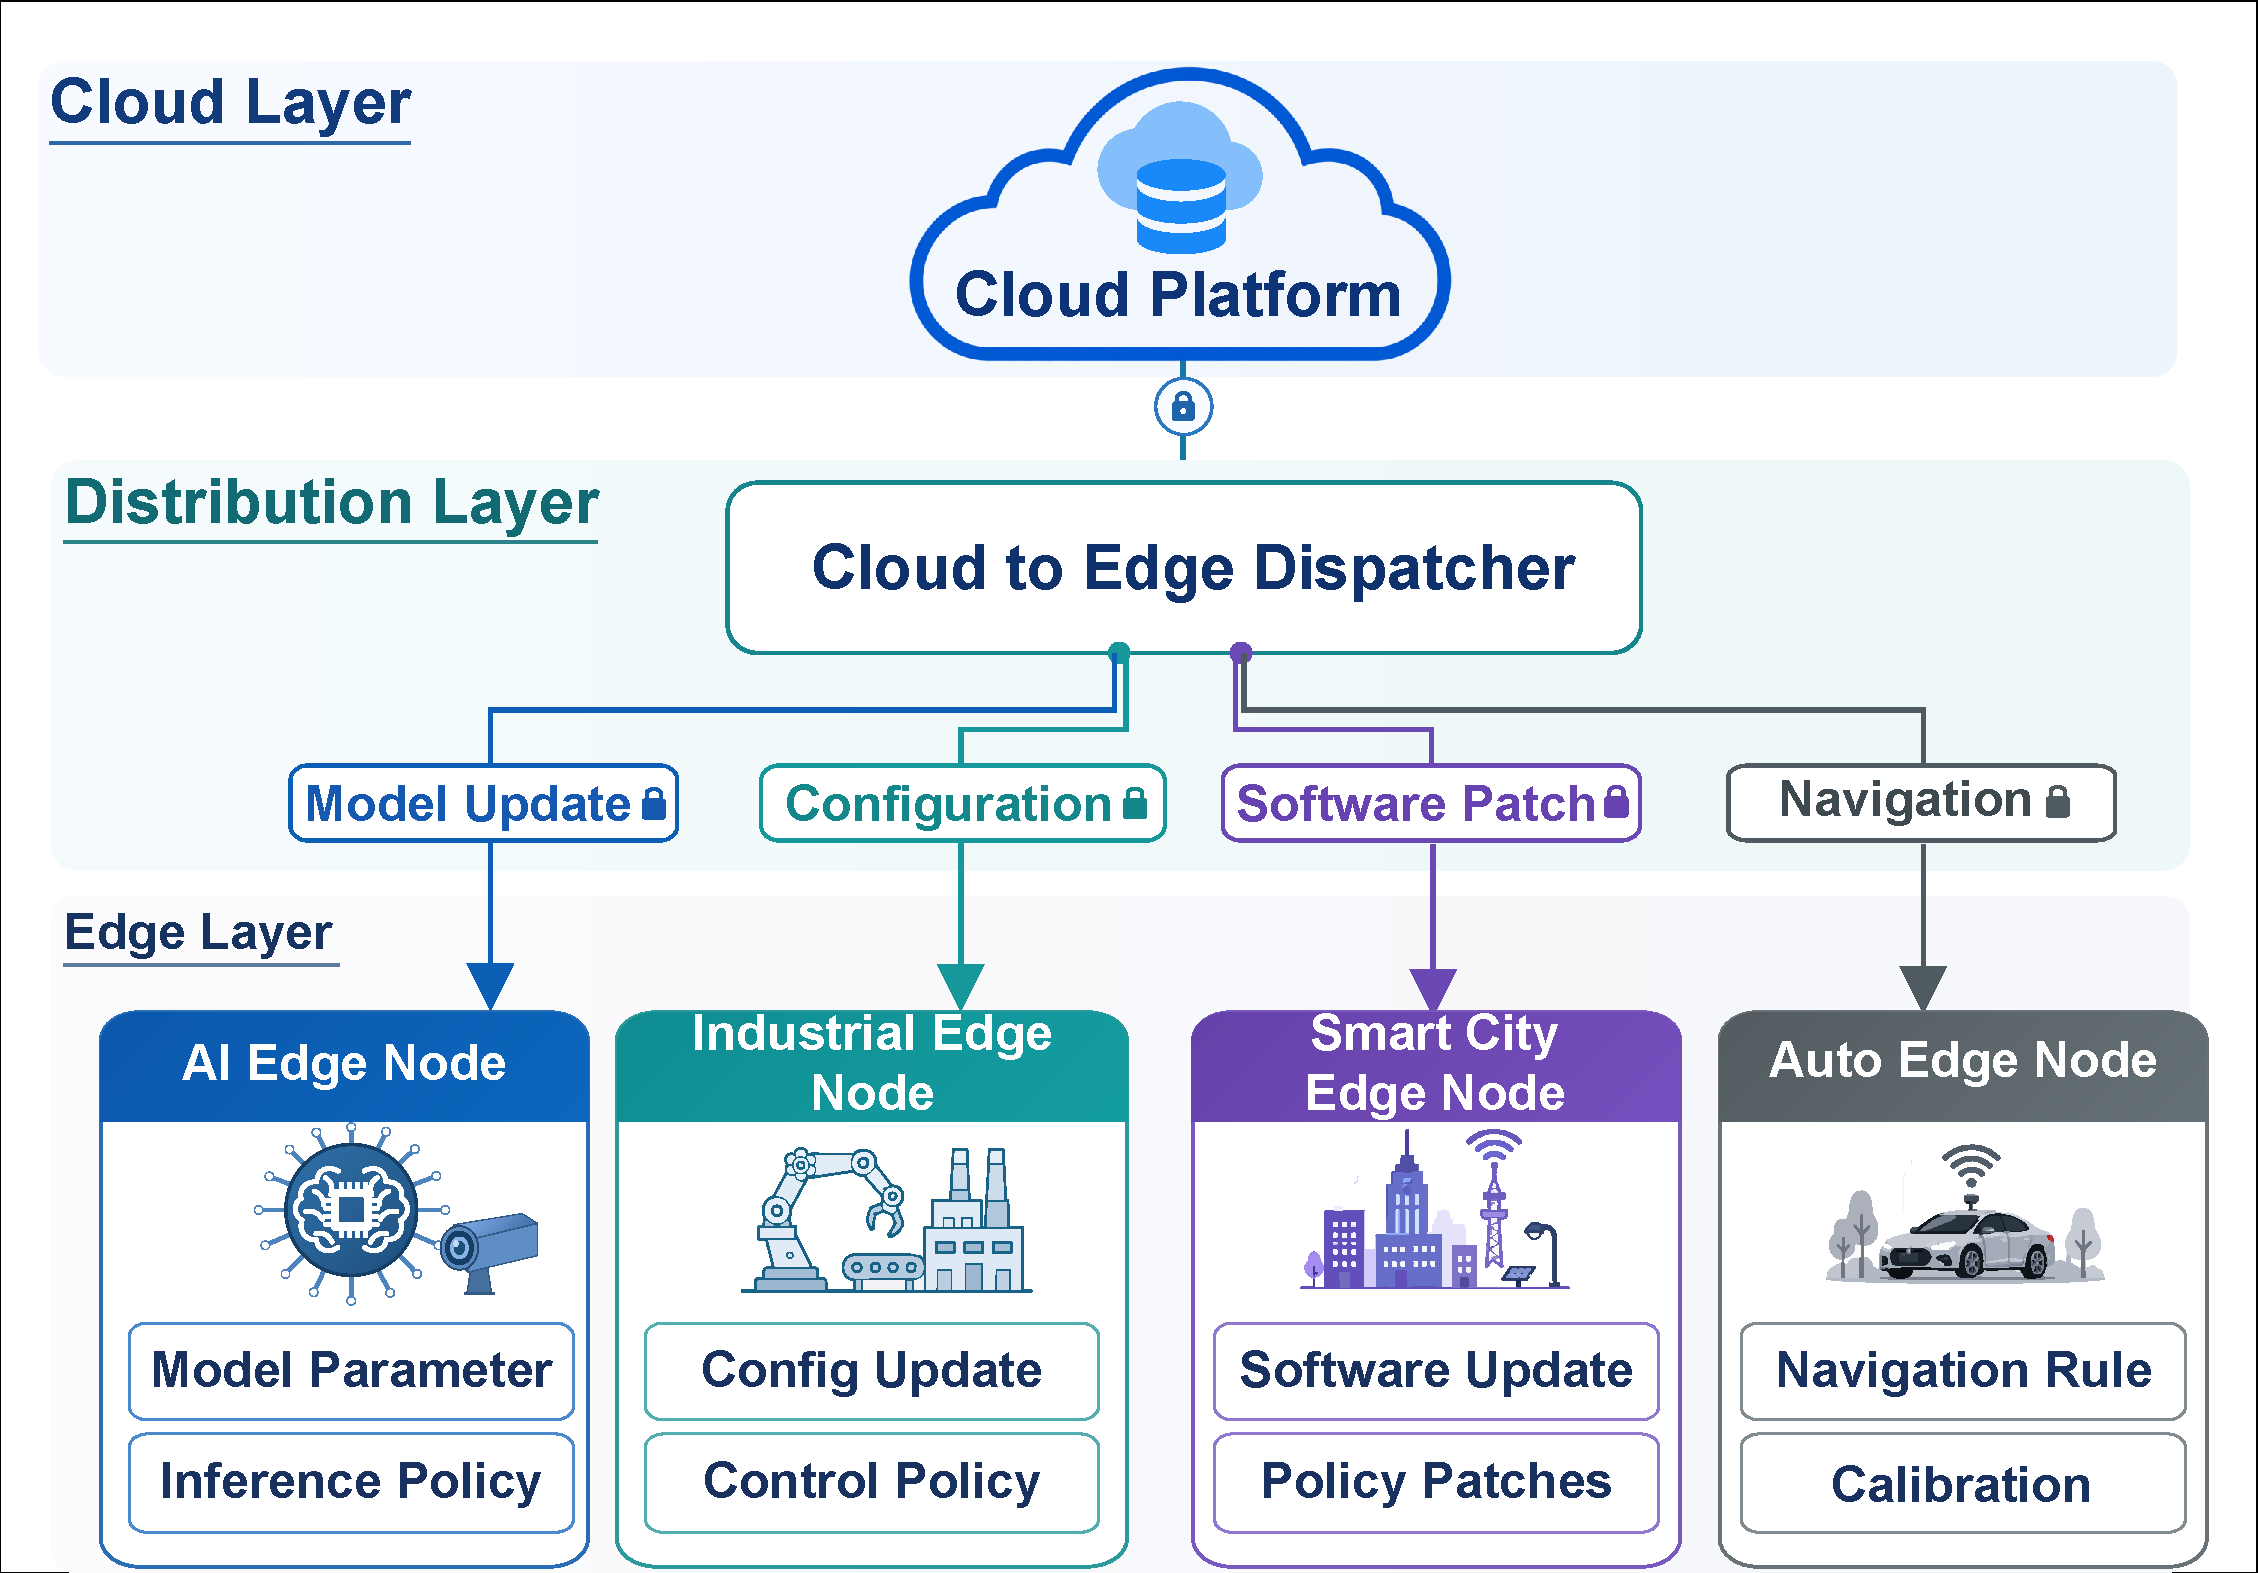
\includegraphics[width=\linewidth]{figures/Edge_Distribution_Aligned.pdf}
	\caption{Cloud-to-edge distribution scenario for edge applications.}
\end{figure}

Cloud-to-edge distribution also faces practical security threats. In 2023, the U.S. Cybersecurity and Infrastructure Security Agency (CISA) reported that 3CXDesktopApp was compromised in a software supply-chain attack \cite{CISA3CX2023}. The incident showed that malicious code can enter trusted software distribution channels. Edge devices themselves are also frequent targets. Microsoft reported a 2026 intrusion that began from an Internet-facing edge appliance \cite{MicrosoftEdge2026}. Such devices may store credentials, certificates, and authentication material. Once compromised, these secrets can be used to access protected systems or data. Therefore, cloud-to-edge distribution should provide confidentiality and source authentication. It should also protect previously distributed data when a current secret key is exposed.

Several cryptographic approaches can be used to meet the security requirements of cloud-to-edge distribution, including signcryption, group key agreement (GKA), and broadcast encryption (BE). Signcryption integrates encryption and digital signatures into a single primitive, providing confidentiality and sender authentication \cite{Zheng1997}. GKA allows multiple users to establish a shared secret key for subsequent data encryption \cite{Ingemarsson1982}. BE allows a sender to encrypt data for a selected set of receivers with a single ciphertext \cite{FiatNaor1993}.

These approaches have different limitations when applied to cloud-to-edge distribution. Conventional signcryption is designed for secure delivery between a sender and a receiver \cite{Zheng1997}. Supporting a large receiver set therefore requires repeated signcryption or an additional broadcast mechanism, which increases the cost at the cloud side. GKA can establish a common key for multiple edge nodes, but it requires key agreement among group members. Dynamic membership also introduces additional key-update operations for joining and leaving nodes \cite{Steiner2000}. This interaction becomes costly when the receiver set changes frequently. BE is more suitable for this setting. It allows the cloud to encrypt once for a selected receiver set without an online group-key negotiation \cite{FiatNaor1993}. The main challenge is to achieve this functionality with compact parameters and strong security. For example, the BGW scheme achieves constant-size ciphertexts and private keys, but its public key grows linearly with the number of users \cite{BGW05}. This tradeoff makes the design of efficient BE schemes a continuing problem.

Key exposure is a serious concern in edge computing. Edge nodes are geographically distributed and may operate outside well-protected cloud infrastructures \cite{ETSIEdgeNative2023}. Their distributed deployment increases the attack surface and may provide weaker physical protection than centralized cloud facilities \cite{NISTIR8320}. A compromised edge node may expose locally stored secret keys. An adversary can then use the leaked key to attack previously recorded ciphertexts. Forward-secure broadcast encryption (FS-BE) limits this risk by evolving receiver keys over time, so that the current key cannot decrypt ciphertexts from earlier periods \cite{yao2004complex,attrapadung2006forward}. This property is particularly useful for cloud-to-edge distribution, where software, models, and configurations may be delivered repeatedly over the lifetime of an edge node. Distributed broadcast encryption (DBE) further removes centralized user-key generation and allows edge nodes to generate their own key pairs \cite{kolonelos2023distributed}. However, existing DBE schemes rely on static receiver keys and do not provide protection for past ciphertexts after key exposure. To the best of our knowledge, no forward-secure DBE construction has been proposed. This leaves a gap for edge systems that require both distributed key management and protection of previously distributed data.

In this work, we propose forward-secure distributed broadcast signcryption (FS-DBS) for cloud-to-edge distribution. FS-DBS supports independent user key generation and selective one-to-many delivery. Receiver keys evolve across time periods, preventing exposure of a current key from compromising earlier ciphertexts. Sender authentication is incorporated into the signcryption process. The ciphertext size remains constant with respect to the receiver set and the system size.

Our main contributions are summarized as follows.

\begin{itemize}
	
	\item \textbf{Forward-secure distributed broadcast signcryption.}
	We construct a distributed broadcast signcryption scheme with receiver-key evolution. User keys are generated independently without a centralized key-generation authority, and expired receiver states are erased after each update.
	
	\item \textbf{Constant-size ciphertext and chosen-ciphertext security.}
	The ciphertext contains a constant number of group elements. We prove selective FS-IND-CCA confidentiality and selective EUF-CMA unforgeability in the random oracle model under the dBDHE assumption.
	
	\item \textbf{Receiver-set-independent online computation.}
	With receiver-set-dependent values computed offline, Signcrypt and Unsigncrypt each use a constant number of online group operations. We evaluate these costs over BLS12-381 for receiver sets of up to 1,000 users.
	
\end{itemize}


\section{Related Work}

In this section, we introduce two areas related to FS-DBS: broadcast encryption and forward-secure encryption.
\subsection{Broadcast Encryption}
Broadcast encryption was introduced by Fiat and Naor~\cite{FiatNaor1993} to enable a sender to encrypt a message for a selected subset of users over a broadcast channel. A central objective in subsequent work has been to reduce communication and storage overhead while preserving collusion resistance. Stateless subset-cover techniques support receiver revocation without requiring receivers to maintain synchronized state~\cite{naor2001revocation}. Boneh, Gentry, and Waters~\cite{BGW05} proposed a pairing-based construction with constant-size ciphertexts and private keys, at the cost of public parameters linear in the maximum number of users. Delerabl\'ee obtained identity-based broadcast encryption with constant-size ciphertexts and private keys~\cite{delerablee2007ibbe}. Later work strengthened the security guarantees of compact BE. Gentry and Waters~\cite{gentry2009adaptive} developed techniques for adaptive security with short ciphertexts, while Phan et al.~\cite{phan2012cca} constructed a broadcast encryption scheme achieving selective chosen-ciphertext security with constant-size ciphertexts and secret keys. These constructions provide efficient one-to-many confidentiality, but user secret keys are generated from centralized secret information.

DBE removes this key-generation dependency by allowing users to generate their own key pairs. Kolonelos, Malavolta, and Wee~\cite{kolonelos2023distributed} formalized efficient DBE from standard assumptions in prime-order bilinear groups and obtained adaptively secure constructions whose ciphertext size is independent of the receiver-set size. Their approach eliminates the key-escrow problem of conventional BE while retaining efficiency comparable to pairing-based broadcast encryption. More recently, Champion and Wu~\cite{champion2024distributed} constructed DBE from lattice assumptions, extending the primitive beyond pairing-based settings. Lee~\cite{lee2025cca} further investigated chosen-ciphertext security for DBE and proposed constructions with constant-size ciphertexts under an adaptive chosen-ciphertext attack (CCA) model. These works substantially strengthen the trust and security properties of BE, but the receiver secret keys remain static across the lifetime of the system. Consequently, compromise of a receiver key can expose ciphertexts recorded before the compromise.

A parallel line of work incorporates authentication into one-to-many encryption. Signcryption, introduced by Zheng~\cite{Zheng1997}, combines confidentiality and authentication within a single cryptographic operation. Multi-receiver and broadcast signcryption extend this functionality to a set of recipients. Selvi et al.~\cite{selvi2009multireceiver} presented an identity-based multi-receiver signcryption construction with ciphertext size independent of the number of receivers, while subsequent broadcast signcryption schemes considered confidentiality and unforgeability under identity-based settings~\cite{selvi2009broadcast,zhang2011broadcast}. These schemes demonstrate that authentication can be integrated efficiently with broadcast delivery. However, this line of work generally relies on static recipient secret keys and does not provide the independently generated user keys required by DBE together with protection of historical ciphertexts after key exposure. FS-DBS combines these requirements by incorporating sender authentication into a distributed broadcast construction while allowing receiver secret states to evolve over time.
\begin{table*}[htbp]
	\centering
	\caption{Comparison of security and functionality properties of FS-DBS and related schemes.}
	\label{tab:property_comparison}
	\small
	\setlength{\tabcolsep}{3pt}
	\renewcommand{\arraystretch}{1.15}
	
	\begin{tabular*}{\textwidth}{@{\extracolsep{\fill}}lccccccc@{}}
		\toprule
		Scheme &
		Independent Key  &
		Forward Security &
		Authentication &
		CCA &
		Constant Ciphertext &
		Non-Interactive Update &
		Arbitrary Receiver \\
		\midrule
		
		KMW23~\cite{kolonelos2023distributed}
		& $\checkmark$ & $\times$ & $\times$ & $\times$ & $\checkmark$ & -- & $\checkmark$ \\
		
		Lee25~\cite{lee2025cca}
		& $\checkmark$ & $\times$ & $\times$ & $\checkmark$ & $\checkmark$ & -- & $\checkmark$ \\
		
		AFI06~\cite{attrapadung2006forward}
		& $\times$ & $\checkmark$ & $\times$ & $\checkmark$ & $\checkmark$ & $\checkmark$ & $\checkmark$ \\
		
		Li17-AAGKA~\cite{li2017aagka}
		& $\times$ & $\checkmark$ & $\checkmark$ & $\checkmark$ & $\checkmark$ & $\times$ & $\times$ \\
		
		Zhang23-DAAGKA~\cite{zhang2023daagka}
		& $\times$ & $\checkmark$ & $\checkmark$ & $\checkmark$ & $\checkmark$ & $\times$ & $\times$ \\
		
		\midrule
		\textbf{FS-DBS}
		& $\checkmark$ & $\checkmark$ & $\checkmark$ & $\checkmark$ & $\checkmark$ & $\checkmark$ & $\checkmark$ \\
		
		\bottomrule
	\end{tabular*}
\end{table*}
\subsection{Forward-Secure Encryption}

Forward security addresses the long-term consequences of secret-key exposure. Bellare and Miner formalized forward security for evolving digital signatures~\cite{bellare1999forward}, while key-insulated cryptography limits exposure by separating periodically refreshed key material from a protected helper~\cite{dodis2002keyinsulated}. Canetti, Halevi, and Katz~\cite{canetti2003forward} introduced the first non-interactive forward-secure public-key encryption constructions. Their approach divides the lifetime of a system into time periods and evolves the secret key such that exposure of the current key does not compromise ciphertexts from previous periods. Tree-based key evolution provides an efficient realization of this principle by associating secret states with nodes of a hierarchical time structure, allowing the storage and update costs to grow only logarithmically with the number of supported periods. Related hierarchical encryption techniques were subsequently developed to obtain compact ciphertexts and efficient delegation, and were shown to support forward-secure encryption as an application~\cite{yao2004complex,boneh2005hierarchical}.

Forward security has also been considered in the broadcast setting. Attrapadung, Furukawa, and Imai~\cite{attrapadung2006forward} proposed forward-secure and searchable broadcast encryption with short ciphertexts and private keys. Their construction combines broadcast encryption with hierarchical key evolution so that a secret key exposed in a later period cannot decrypt ciphertexts from earlier periods. This establishes that forward security can be achieved without sacrificing compact broadcast ciphertexts. However, existing forward-secure broadcast constructions retain the conventional broadcast-encryption model in which receiver credentials originate from centralized key-generation material, and they do not simultaneously address distributed user-key generation and sender authentication.

FS-DBS builds on these complementary directions. It retains the independently generated user keys of DBE while introducing time-dependent receiver secret states and erasure of expired key material. At the same time, authentication is incorporated into the broadcast ciphertext rather than provided through a separate signature layer. The resulting construction therefore targets a setting in which receiver-key exposure, centralized key escrow, and unauthenticated distribution must be addressed simultaneously, while keeping the cryptographic ciphertext size independent of the receiver-set size.

Li et al.~\cite{li2017aagka} proposed authenticated asymmetric group key
agreement (AAGKA) with sender non-repudiation and privacy. Zhang et
al.~\cite{zhang2023daagka} later proposed a dynamic authenticated asymmetric
group key agreement (DAAGKA) protocol. We use the labels Li17-AAGKA and
Zhang23-DAAGKA in tables and figures.


Table~\ref{tab:property_comparison} compares the security and functional properties of other schemes. DBE schemes support independent key generation but lack forward security, while AFI06 provides forward security without distributed key generation or authentication. AAGKA schemes provide forward security and authentication but require interaction for period updates. FS-DBS combines these properties without interactive period updates while retaining constant-size ciphertexts.

\section{Preliminaries}
	This section introduces the bilinear group and hardness assumptions
underlying our construction.
\subsection{Bilinear Groups and Assumptions}
Assume a bilinear group setting $\mathsf{bg}:= (p, \mathbb{G}_{1}, \mathbb{G}
_{2}, \mathbb{G}_{T}, $ $g_{1}, g_{2}, e)$, where $p$ is a prime of $\lambda$-bit
length, $\mathbb{G}_{1}$, $\mathbb{G}_{2}$, and $\mathbb{G}_{T}$ are cyclic groups
of prime order $p$. Pairing-friendly prime-order curves provide practical
instantiations of this setting~\cite{barreto2006pairing}. For any
$m\in\mathbb{Z}_p$, let $[m]_1:=g_1^m$ and $[m]_2:=g_2^m$. Define $g_T:=e(g_1,g_2)$ and $[m]_T:=g_T^m$.
Let $e$ denote a bilinear pairing. It satisfies:


\begin{enumerate}
	\item \textbf{Bilinearity}: For all $a,b\in\mathbb{Z}_p$,
	\begin{equation*}
		e([a]_1,[b]_2)=e([1]_1,[1]_2)^{ab}
	\end{equation*}
	
	\item \textbf{Non-degeneracy}:
	\begin{equation*}
		e([1]_{1}, [1]_{2}) \neq 1
	\end{equation*}
	
	\item \textbf{Efficient computability}: The pairing $e$ can be computed efficiently.
\end{enumerate}

Under this setting, the security of FS-DBS relies on the decisional Bilinear Diffie--Hellman Exponent (dBDHE) assumption.

\begin{assumption}[$q$-dBDHE]
	Let $\mathcal{BG}$ be a bilinear-group generator. Sample
	$\mathsf{bg}\overset{\$}{\leftarrow}\mathcal{BG}(1^\lambda)$ and
	$\alpha,s\overset{\$}{\leftarrow}\mathbb{Z}_p^*$, and define
	\[
	\mathcal{D}_q=
	\left(
	\{[\alpha^j]_1\}_{j\in[q]},
	\{[\alpha^j]_2\}_{j\in[2q],\,j\neq q+1},
	[s]_1
	\right).
	\]
	Let $T_0=[s\alpha^{q+1}]_T$ and sample
	$T_1\overset{\$}{\leftarrow}\mathbb{G}_T$. The $q$-dBDHE
	assumption holds if, for every PPT adversary $\mathcal{A}$,
	\[
	\begin{aligned}
	\operatorname{Adv}^{\mathsf{dBDHE}}_{\mathcal{BG},q,\mathcal{A}}(\lambda)
	&=
	\left|
	\Pr[\mathcal{A}(\mathsf{bg},\mathcal{D}_q,T_0)=1]
	-
	\Pr[\mathcal{A}(\mathsf{bg},\mathcal{D}_q,T_1)=1]
	\right|\\
	&\leq \operatorname{negl}(\lambda).
	\end{aligned}
	\]
\end{assumption}
\subsection{Binary Time Tree and Forward Security}

Following the tree-based key-evolution approach~\cite{canetti2003forward,attrapadung2006forward}, we represent time periods by nodes of a binary tree of depth $d$. A node at depth $z$ is denoted by
\[
w=(w_1,\ldots,w_z)\in\{1,2\}^z,\qquad 0\leq z\leq d
\]
where the root is denoted by $\epsilon$. For a node $w$, its two children are $w\|1$ and $w\|2$. For comparisons between nodes at different depths, we use the canonical padded representation
\[
\widehat{w}=(w_1,\ldots,w_z,0^{d-z})\in\{0,1,2\}^{d}.
\]
The symbol $0$ is used only for padding and is not a time-tree branch label. Each user $i$ maintains an evolving secret state $\mathsf{SK}_{i,w}$ associated with the current time node.

Forward security limits the effect of secret-key exposure across time periods~\cite{canetti2003forward}. The secret key is updated when the system moves from the current node $w$ to a child node $w\|b$, where $b\in\{1,2\}$. After the update, secret material associated with the expired state is erased. In a forward-secure broadcast setting, exposure of $\mathsf{SK}_{i,w'}$ at a later period $w'$ should not enable an adversary to decrypt ciphertexts generated for an earlier period $w$~\cite{attrapadung2006forward}. This property allows receivers to remain secure against retrospective decryption even if their current secret states are eventually compromised.

\section{FS-DBS Scheme}

\begin{figure*}[!t]
	\centering
	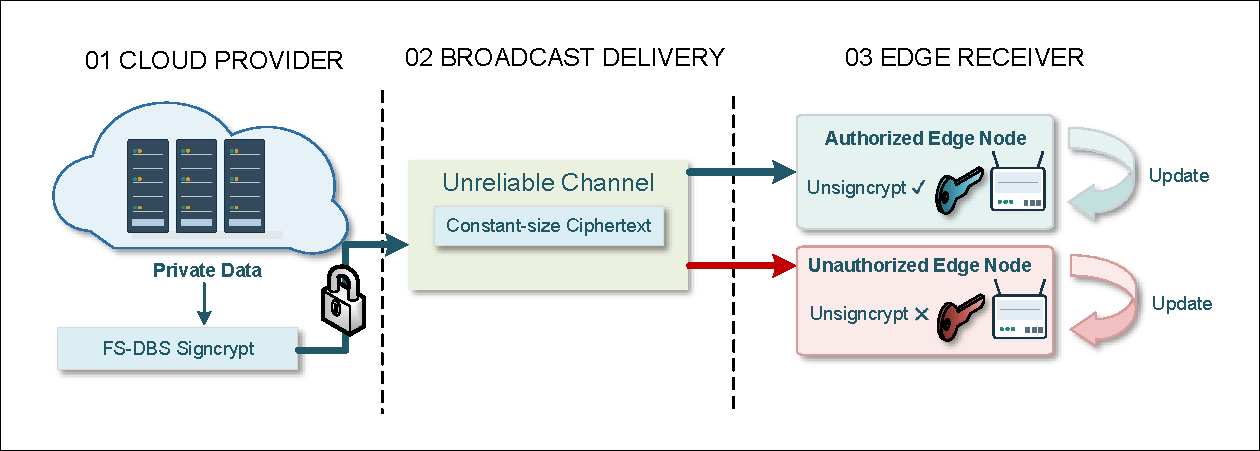
\includegraphics[width=\textwidth]{figures/FSDBS_System_Framework.pdf}
	\caption{FS-DBS workflow for cloud-to-edge distribution and receiver-state evolution. The cloud provider broadcasts a constant-size ciphertext to the selected receivers. Authorized edge nodes verify and decrypt the ciphertext and update their secret states, while unauthorized nodes cannot recover the plaintext.}
	\Description{The cloud provider signcrypts a data release and broadcasts
		the ciphertext through an untrusted delivery network. Authorized edge
		nodes verify and decrypt the ciphertext, update their secret states,
		and erase expired states. A later exposed state cannot recover the
		recorded ciphertext from an earlier period.}
	\label{fig:fsdbs_system_framework}
\end{figure*}
\FloatBarrier

Figure~\ref{fig:fsdbs_system_framework} summarizes the cloud-to-edge
distribution workflow and the receiver-state transition. We next describe
FS-DBS, denoted by $\Pi_{\mathsf{FS\mbox{-}DBS}}$. Let
$H_0:\mathbb{G}_T\rightarrow\mathbb{G}_T$ and
$H_1:\{0,1\}^{*}\rightarrow\mathbb{Z}_{p}\setminus\{0,1,2\}$ be hash
functions modeled as random oracles. Let $n$ be the maximum number of
users and $d$ the depth of the binary time tree, where $d+1\leq n$.
The message space is $\mathbb{M}=\mathbb{G}_T$.
For each time period, let
$w=(w_1,\ldots,w_z)\in\{1,2\}^{z}$, $0\leq z\leq d$, denote its
corresponding tree node. The additional $(d+1)$-th hierarchical level
is reserved for authentication and is not used as a time-tree level.

\noindent$\bullet$ \textbf{Setup}$(1^\lambda,1^n,1^d)$:
On input the security parameter $\lambda$, the number of user slots $n$,
and the time-tree depth $d$, the algorithm generates
$\mathsf{bg}:=(p,\mathbb{G}_1,\mathbb{G}_2,\mathbb{G}_T,
[1]_1,[1]_2,e)\leftarrow\mathsf{BG}(1^\lambda)$ and samples
$\alpha,y\overset{\$}{\leftarrow}\mathbb{Z}_p^{*}$.
Define $Y_1=[y]_1$ and $Y_2=[y]_2$. It outputs:
\[
pp=
\left(
\mathsf{bg},
\{[\alpha^q]_1\}_{q\in[n]},
\{[\alpha^q]_2\}_{q\in[2n],\,q\neq n+1},
Y_1,Y_2,H_0,H_1
\right)
\]
The setup values $\alpha$ and $y$ are then erased.

\noindent$\bullet$ \textbf{Join}$(pp,i)$:
User $i$ samples $t_i,\rho\overset{\$}{\leftarrow}\mathbb{Z}_p^{*}$
and generates the temporary secret key and public key as follows:
\[
\begin{aligned}
	usk_i
	&=
	[t_i\alpha^{n+1-i}]_2
	\\
	upk_i
	&=
	\left(
	[t_i]_1,
	\{[t_i\alpha^q]_2\}_{q\in[n],\,q\neq n+1-i}
	\right)
\end{aligned}
\]
Using $usk_i$, the user initializes its root evolving secret key:
\[
\mathsf{SK}_{i,\epsilon}
=
\left(
[t_i\alpha^{n+1-i}+\rho y]_2,
[\rho]_2,
\{[\rho\alpha^{n+1-\ell}]_2\}_{\ell=1}^{d+1}
\right)
\]
Afterwards, $t_i$ and $usk_i$ are permanently erased, and the algorithm
outputs $(upk_i,\mathsf{SK}_{i,\epsilon})$.

Before registration, the authenticated directory runs \textsf{IsValid} on
$(pp,i,upk_i)$. It parses
$upk_i=(upk_{i,0},\{upk_{i,q}\}_{q\in[n],\,q\neq n+1-i})$
and checks that $upk_{i,0}$ is a nonidentity element of $\mathbb{G}_1$,
and that every $upk_{i,q}$ belongs to $\mathbb{G}_2$. For each
$q\in[n]\setminus\{n+1-i\}$, it checks
\[
e\left([\alpha^{n-q}]_1,upk_{i,q}\right)
=
e\left(upk_{i,0},[\alpha^n]_2\right).
\]
The algorithm returns $1$ only if all checks hold. As in KMW23~\cite{kolonelos2023distributed}, these pairing equations ensure that all public-key coordinates contain the same exponent $t_i$; invalid public keys are rejected before they are added to the directory.

\noindent$\bullet$ \textbf{KeyUpdate}
$(pp,w,\mathsf{SK}_{i,w},b)$:
Let $w=(w_1,\ldots,w_z)$ with $z<d$, and let $b\in\{1,2\}$ be the
next time-tree label. Parse
$\mathsf{SK}_{i,w}=(a_0,a_1,\{b_\ell\}_{\ell=z+1}^{d+1})$ and sample
$\delta\overset{\$}{\leftarrow}\mathbb{Z}_p$. The secret key for the
child node $w\|b$ is generated as follows:
\[
\begin{aligned}
	a_0'
	&=
	a_0\,b_{z+1}^{\,b}
	\left[
	y+
	\sum_{\ell=1}^{z}
	w_\ell\alpha^{n+1-\ell}
	+
	b\alpha^{n-z}
	\right]_2^{\delta}
	\\
	a_1'
	&=
	a_1[\delta]_2
	\\
	b_\ell'
	&=
	b_\ell[\alpha^{n+1-\ell}]_2^{\delta},
	\qquad
	\ell=z+2,\ldots,d+1
\end{aligned}
\]
The algorithm outputs
$\mathsf{SK}_{i,w\|b}
=(a_0',a_1',\{b_\ell'\}_{\ell=z+2}^{d+1})$
and erases the expired secret-key material.

\noindent$\bullet$ \textbf{Signcrypt}
with input $(pp,i,S,\mathsf{SK}_{i,w},w,M)$ and the public-key set
$\{upk_j\}_{j\in S}$:
Parse $\mathsf{SK}_{i,w}=(a_0,a_1,b_{z+1},\ldots)$.
Define
\[
\begin{aligned}
X_S
&=\prod_{j\in S}(upk_{j,0}[\alpha^j]_1),\\
Z_{w,1}
&=Y_1\prod_{\ell=1}^{z}[\alpha^{n+1-\ell}]_1^{w_\ell},\\
Z_{w,2}
&=Y_2\prod_{\ell=1}^{z}[\alpha^{n+1-\ell}]_2^{w_\ell}.
\end{aligned}
\]
Sample $s\overset{\$}{\leftarrow}\mathbb{Z}_p^{*}$ and
$\delta\overset{\$}{\leftarrow}\mathbb{Z}_p$. Compute
\[
\begin{aligned}
	C_0
	&=
	[s]_1
	&
	C_1
	&=
	X_S^s
	=
	\left[
	s\sum_{j\in S}(t_j+\alpha^j)
	\right]_1
	\\
	C_2
	&=
	Z_{w,1}^{\,s}
	&
	C_3
	&=
	a_1[\delta]_2
\end{aligned}
\]
The sender resamples $\delta$ until $C_3\neq 1_{\mathbb{G}_2}$.
Set $K=e([\alpha]_1,[\alpha^n]_2)^s=[s\alpha^{n+1}]_T$ and
$C_5=H_0(K)\cdot M$. The authentication challenge is then computed as:
\[
h=
H_1\left(
i\parallel S\parallel w\parallel
C_0\parallel C_1\parallel C_2\parallel C_3\parallel
C_5\parallel K
\right)
\]
Using $h$, compute
\[
C_4
=
a_0\,b_{z+1}^{\,h}
\left(
Z_{w,2}[\alpha^{n-z}]_2^{\,h}
\right)^{\delta}
\]
Return the ciphertext
\[
ct=(C_0,C_1,C_2,C_3,C_4,C_5)
\]

\noindent$\bullet$ \textbf{Unsigncrypt}
with input $(pp,i,S,k,\mathsf{SK}_{k,w},w,ct)$ and the public-key set
$\{upk_j\}_{j\in S}$:
Parse $ct=(C_0,C_1,C_2,C_3,C_4,C_5)$ and
$\mathsf{SK}_{k,w}=(a_{k,0},a_{k,1},\ldots)$.
If $C_3=1_{\mathbb{G}_2}$, return $\perp$. Otherwise, define
\[
\begin{aligned}
Z_{w,1}
&=Y_1\prod_{\ell=1}^{z}[\alpha^{n+1-\ell}]_1^{w_\ell},\\
Y
&=a_{k,0}\prod_{\substack{j\in S\\j\neq k}}
\left(upk_{j,n+1-k}[\alpha^{n+1+j-k}]_2\right).
\end{aligned}
\]
The receiver first computes
\[
K=
e(C_1,[\alpha^{n+1-k}]_2)
e(C_2,a_{k,1})
e(C_0,Y)^{-1}
\]
The authentication challenge is then computed as:
\[
h=
H_1\left(
i\parallel S\parallel w\parallel
C_0\parallel C_1\parallel C_2\parallel C_3\parallel
C_5\parallel K
\right)
\]
The ciphertext is accepted only if the following pairing relation
holds:
\[
e([1]_1,C_4)
=
e\left(
upk_{i,0},
[\alpha^{n+1-i}]_2
\right)
e\left(
Z_{w,1}[\alpha^{n-z}]_1^{\,h},
C_3
\right)
\]
If the equality does not hold, the algorithm returns $\perp$.
Otherwise, the plaintext is recovered as
$M=C_5H_0(K)^{-1}$.


\subsection{Offline Precomputation}

For a fixed receiver set $S$ and time node $w$, part of the computation required by Signcrypt and Unsigncrypt is already determined before the message is available. These values can be computed in advance and reused during the online phase. We discuss the precomputation for Signcrypt and Unsigncrypt separately below.

\noindent\textbf{Signcrypt.}
Once $S$ and $w$ are fixed, the sender precomputes
\[
\left(
X_S,
Z_{w,1},
Z_{w,2},
[\alpha^{n-z}]_2
\right)
\]
These values are independent of the message $M$ and randomness. During the online phase, the sender only samples $s$ and $\delta$ and generates $C_0,\ldots,C_5$ using the precomputed values and the current secret state. The number of online group operations is constant and independent of $|S|$.

\noindent\textbf{Unsigncrypt.}
The receiver can also precompute the terms that depend on the receiver set and the registered sender. For receiver $k$ and sender $i$, define
\[
\begin{aligned}
	Y_{k,S}
	&=
	a_{k,0}
	\prod_{\substack{j\in S\\j\neq k}}
	\left(
	upk_{j,n+1-k}
	[\alpha^{n+1+j-k}]_2
	\right) \\
	V_i
	&=
	e\left(
	upk_{i,0},
	[\alpha^{n+1-i}]_2
	\right)
\end{aligned}
\]
The value $Y_{k,S}$ is refreshed when $S$ or the receiver secret state changes, while $V_i$ can be reused for the same sender. With these values available, Unsigncrypt performs a fixed number of pairing operations during the online phase.



\subsection{Correctness}

We show that the key-update, authentication, and decryption procedures
are correct.

\paragraph{Correctness of KeyUpdate.}
Assume that the secret key associated with
$w=(w_1,\ldots,w_z)$ has the following algebraic form:
\[
\begin{aligned}
	a_0
	&=
	\left[
	t_i\alpha^{n+1-i}
	+
	\rho
	\left(
	y+\sum_{\ell=1}^{z}
	w_\ell\alpha^{n+1-\ell}
	\right)
	\right]_2
	\\
	a_1
	&=
	[\rho]_2
	\\
	b_\ell
	&=
	[\rho\alpha^{n+1-\ell}]_2,
	\qquad
	\ell=z+1,\ldots,d+1
\end{aligned}
\]
For a child label $b\in\{1,2\}$, the first updated component satisfies:
\[
\begin{aligned}
	a_0'
	&=
	a_0\,b_{z+1}^{\,b}
	\left[
	y+
	\sum_{\ell=1}^{z}
	w_\ell\alpha^{n+1-\ell}
	+
	b\alpha^{n-z}
	\right]_2^\delta
	\\
	&=
	\left[
	t_i\alpha^{n+1-i}
	+
	(\rho+\delta)
	\left(
	y+
	\sum_{\ell=1}^{z}
	w_\ell\alpha^{n+1-\ell}
	+
	b\alpha^{n-z}
	\right)
	\right]_2
\end{aligned}
\]
The remaining components satisfy:
\[
a_1'=[\rho+\delta]_2,
\qquad
b_\ell'=
[(\rho+\delta)\alpha^{n+1-\ell}]_2,
\quad
\ell=z+2,\ldots,d+1
\]
Hence, the resulting state has exactly the required form for the child
node $w\|b$ with fresh effective randomness $\rho+\delta$.

\paragraph{Correctness of Authentication.}
For sender $i$ and the current time node $w$, write the evolving
secret-key components in the following form:
\[
\begin{aligned}
	a_0
	&=
	\left[
	t_i\alpha^{n+1-i}
	+
	\rho
	\left(
	y+
	\sum_{\ell=1}^{z}
	w_\ell\alpha^{n+1-\ell}
	\right)
	\right]_2
	\\
	a_1
	&=
	[\rho]_2
	&
	b_{z+1}
	&=
	[\rho\alpha^{n-z}]_2
\end{aligned}
\]
The value $t_i$ is used here only to express the algebraic form of the
evolving secret key and has already been erased after \textbf{Join}.
From the definition of $C_3$, we obtain:
\[
C_3
=
a_1[\delta]_2
=
[\rho+\delta]_2
\]
Expanding $C_4$ gives
\[
\begin{aligned}
	C_4
	&=
	a_0\,b_{z+1}^{\,h}
	\left(
	Z_{w,2}[\alpha^{n-z}]_2^{\,h}
	\right)^\delta
	\\
	&=
	\left[
	t_i\alpha^{n+1-i}
	+
	(\rho+\delta)
	\left(
	y+
	\sum_{\ell=1}^{z}
	w_\ell\alpha^{n+1-\ell}
	+
	h\alpha^{n-z}
	\right)
	\right]_2
\end{aligned}
\]
Using the bilinearity of $e$, the verification equation becomes:
\[
\begin{aligned}
	e([1]_1,C_4)
	&=
	e\left(
	[t_i]_1,
	[\alpha^{n+1-i}]_2
	\right)
	\\
	&\quad\cdot
	e\left(
	\left[
	y+
	\sum_{\ell=1}^{z}
	w_\ell\alpha^{n+1-\ell}
	+
	h\alpha^{n-z}
	\right]_1,
	[\rho+\delta]_2
	\right)
	\\
	&=
	e\left(
	upk_{i,0},
	[\alpha^{n+1-i}]_2
	\right)
	e\left(
	Z_{w,1}[\alpha^{n-z}]_1^{\,h},
	C_3
	\right)
\end{aligned}
\]
Therefore, every honestly generated ciphertext passes the
authentication check.

\paragraph{Correctness of Decryption.}
For receiver $k\in S$ and the current time node $w$, write its evolving
secret-key components in the following form:
\[
\begin{aligned}
	a_{k,0}
	&=
	\left[
	t_k\alpha^{n+1-k}
	+
	\rho
	\left(
	y+
	\sum_{\ell=1}^{z}
	w_\ell\alpha^{n+1-\ell}
	\right)
	\right]_2
	\\
	a_{k,1}
	&=
	[\rho]_2
\end{aligned}
\]
Using the definitions of $C_1$, $C_2$, and $a_{k,1}$, the first two
terms of the decryption equation expand to:
\[
\begin{aligned}
	&e(C_1,[\alpha^{n+1-k}]_2)e(C_2,a_{k,1})
	\\
	&=
	\Bigg[
	s\sum_{j\in S}
	\left(
	t_j\alpha^{n+1-k}
	+
	\alpha^{n+1+j-k}
	\right)
	+
	s\rho
	\left(
	y+
	\sum_{\ell=1}^{z}
	w_\ell\alpha^{n+1-\ell}
	\right)
	\Bigg]_T
\end{aligned}
\]
On the other hand, the cancellation term derived from $Y$ is:
\[
\begin{aligned}
	e(C_0,Y)
	=
	\Bigg[
	s\Bigg(
	&t_k\alpha^{n+1-k}
	+
	\rho
	\left(
	y+
	\sum_{\ell=1}^{z}
	w_\ell\alpha^{n+1-\ell}
	\right)
	\\
	&+
	\sum_{\substack{j\in S\\j\neq k}}
	\left(
	t_j\alpha^{n+1-k}
	+
	\alpha^{n+1+j-k}
	\right)
	\Bigg)
	\Bigg]_T
\end{aligned}
\]
All terms involving $t_j$ and the time-dependent randomization cancel.
The only remaining contribution corresponds to $j=k$:
\[
\alpha^{n+1+k-k}=\alpha^{n+1}
\]
Consequently,
\[
\begin{aligned}
	K
	&=
	e(C_1,[\alpha^{n+1-k}]_2)
	e(C_2,a_{k,1})
	e(C_0,Y)^{-1}
	\\
	&=
	[s\alpha^{n+1}]_T
\end{aligned}
\]
This value of $K$ is identical to that computed by \textbf{Signcrypt}.
Since $C_5=H_0(K)\cdot M$, the receiver obtains
$M=C_5H_0(K)^{-1}$.
\section{Security Analysis}
We first define the security and threat model of FS-DBS, and then prove its selective FS-IND-CCA confidentiality and selective EUF-CMA unforgeability.



\subsection{Threat Model}

FS-DBS is designed for periodic data distribution from a cloud provider to distributed edge nodes. The cloud provider acts as the sender, while the selected edge nodes form the receiver set. Each participant generates its own key through \textsf{Join}. The authenticated directory registers the public key only if \textsf{IsValid} returns $1$. The setup algorithm does not generate or retain user secret keys.

Edge nodes may operate outside well-protected cloud environments and remain deployed for long periods. We therefore allow an adversary to compromise receiver nodes and obtain the secret state stored on the device. The adversary may also control receivers outside the target set and combine the exposed states of multiple nodes. In the forward-security setting, a target receiver may be compromised after the protected period. The adversary can retain ciphertexts observed before the compromise and use the exposed state in later attacks.

The cloud-to-edge delivery channel is untrusted. The adversary can record, delay, modify, and inject ciphertexts. The target cloud sender is not compromised. An honest edge node erases its expired secret state and the corresponding update randomness after \textsf{KeyUpdate}. This erasure is required for forward security. Denial of service, traffic analysis, side-channel leakage, and rollback of the application-level period counter are outside the model. The receiver checks the time node carried by a ciphertext against its local period before decryption.

\subsection{Security Model}

Let $\mathcal{T}$ denote the set of time nodes. For $w,v\in\mathcal{T}$, we write $w\prec v$ if $v$ is reached from $w$ by one or more calls to \textsf{KeyUpdate}; hence, $v$ is a strict descendant of $w$. The relation $w\preceq v$ also allows $w=v$. Although an expired state is erased by an honest receiver, we use $\mathsf{SK}_{i,w}$ to denote the secret state associated with user $i$ at time node $w$.

\noindent\textbf{Oracle Interface.}
Both security experiments provide consistent access to the random oracles $H_0$ and $H_1$. The signcryption oracle $\mathcal{O}_{\mathrm{SC}}(i,S,w,M)$ returns an honestly generated ciphertext for sender $i$, receiver set $S$, time node $w$, and message $M$. The unsigncryption oracle $\mathcal{O}_{\mathrm{USC}}(i,S,w,j,ct)$ runs \textsf{Unsigncrypt} with $\mathsf{SK}_{j,w}$ and returns either the recovered message or $\bot$. The exposure oracle $\mathcal{O}_{\mathrm{Exp}}(j,v)$ returns $\mathsf{SK}_{j,v}$. The admissible exposure queries are specified separately in each experiment.

\noindent\textbf{Definition 1 (Selective FS-IND-CCA Confidentiality).}
Let $\Pi$ be an FS-DBS scheme. The experiment
$\operatorname{Exp}^{\mathrm{FS\text{-}IND\text{-}CCA}_{\Pi,\mathcal{A}}}(\lambda)$
is defined as follows.

\begin{enumerate}
	\item \textbf{Commit.}
	Before setup, $\mathcal{A}$ commits to a target sender $i^*$, a nonempty receiver set $S^*$ with $i^*\notin S^*$, and a target time node $w^*$.
	
	\item \textbf{Setup.}
	The challenger runs \textsf{Setup} and \textsf{Join} for all registered users and gives the public parameters and registered public keys to $\mathcal{A}$.
	
	\item \textbf{Query 1.}
	The adversary may query $H_0$, $H_1$, $\mathcal{O}_{\mathrm{SC}}$, $\mathcal{O}_{\mathrm{USC}}$, and $\mathcal{O}_{\mathrm{Exp}}$. For every $j\in S^*$, an exposure query $\mathcal{O}_{\mathrm{Exp}}(j,v)$ is allowed only when $w^*\prec v$. Receivers outside $S^*$ may be exposed at any time.
	
	\item \textbf{Challenge.}
	The adversary submits two equal-length messages $M_0$ and $M_1$. The challenger samples $b\sample\{0,1\}$ and returns
	\[
	ct^* \leftarrow
	\textsf{Signcrypt}
	\left(
	pp,i^*,S^*,\mathsf{SK}_{i^*,w^*},w^*,M_b
	\right)
	\]
	
	\item \textbf{Query 2.}
	The adversary continues to access the same oracles under the exposure restriction above. It may not submit $ct^*$ to $\mathcal{O}_{\mathrm{USC}}$ under the target tuple $(i^*,S^*,w^*)$ for any $j\in S^*$.
	
	\item \textbf{Guess.}
	The adversary outputs $b'$. The experiment returns $1$ if $b'=b$ and $0$ otherwise.
\end{enumerate}

The advantage of $\mathcal{A}$ is
\[
\operatorname{Adv}^{\mathrm{FS\text{-}IND\text{-}CCA}_{\Pi,\mathcal{A}}}(\lambda)
=
\left|
\Pr[b'=b]-\frac{1}{2}
\right|
\]

The scheme is selectively FS-IND-CCA secure if this advantage is negligible for every PPT adversary. In particular, the experiment allows the future state of every receiver in $S^*$ to be exposed after $w^*$.

\noindent\textbf{Definition 2 (Selective EUF-CMA Unforgeability).}
Let $\Pi$ be an FS-DBS scheme. The experiment
$\operatorname{Exp}^{\mathrm{EUF\text{-}CMA}_{\Pi,\mathcal{F}}}(\lambda)$
is defined as follows.

\begin{enumerate}
	\item \textbf{Commit.}
	Before setup, $\mathcal{F}$ commits to a target sender $i^*$, a nonempty receiver set $S^*$ with $i^*\notin S^*$, and a time node $w^*$.
	
	\item \textbf{Setup and Queries.}
	The challenger runs \textsf{Setup} and \textsf{Join} and gives the public information to $\mathcal{F}$. The adversary may query $H_0$, $H_1$, $\mathcal{O}_{\mathrm{USC}}$, and the signcryption oracle on messages of its choice under $(i^*,S^*,w^*)$. Receiver states may also be exposed, while the secret state of the target sender is not revealed. Let $Q_{\mathrm{SC}}$ denote the set of messages submitted to the target signcryption oracle.
	
	\item \textbf{Forgery.}
	The adversary outputs a ciphertext $ct^*$. For each $j\in S^*$, the challenger computes
	\[
	M_j^*
	\leftarrow
	\textsf{Unsigncrypt}
	\left(
	pp,i^*,S^*,j,\mathsf{SK}_{j,w^*},w^*,ct^*
	\right)
	\]
	
	\item \textbf{Win.}
	The experiment returns $1$ if there exists $j\in S^*$ such that $M_j^*\neq\bot$ and $M_j^*\notin Q_{\mathrm{SC}}$. Otherwise, it returns $0$.
\end{enumerate}

The advantage of $\mathcal{F}$ is
\[
\operatorname{Adv}^{\mathrm{EUF\text{-}CMA}_{\Pi,\mathcal{F}}}(\lambda)
=
\Pr
\left[
\operatorname{Exp}^{\mathrm{EUF\text{-}CMA}_{\Pi,\mathcal{F}}}(\lambda)=1
\right]
\]

The scheme is selectively EUF-CMA secure if this probability is negligible for every PPT adversary.

The FS-IND-CCA experiment protects data distributed before a later receiver compromise. The EUF-CMA experiment protects the authenticity of data distributed by an uncompromised cloud sender.






\subsection{Security Proofs}

	%%%%%%%%%%%%%%%%%%%%%%%%%%%%%%%%%%%%%%%%%%%%%%%%%%%%%%%%%%%%%%%%%%%%%%%%%%%%%%%%%%%%%%%%%%%%%
%定理
\begin{theorem}
	\label{theorem:CCA}
	If a PPT adversary $\mathcal{A}$ has a non-negligible advantage
	$\epsilon$ against the selective FS-IND-CCA security of FS-DBS in
	the random oracle model, then there exists a PPT algorithm
	$\mathcal{B}$ that solves the dBDHE problem with advantage at least
	$\epsilon-\frac{q_U}{p-3}-\operatorname{negl}(\lambda)$, where $q_U$
	is the number of unsigncryption-oracle queries.
\end{theorem}
%%%%%%%%%%%%%%%%%%%%%%%%%%%%%%%%%%%%%%%%%%%%%%%%%%%%%%%%%%%%%%%%%%%%%%%%%%%%%%%%%%%%%%%%%%%%%
%证明
\begin{proof}
	%%%%%%%%%%%%%%%%%%%%%%%%%%%%%%%%%%%%%%%%%%%%%%%%%%%%%%%%%%%%%%%%%%%%%%%%%%%%%%%%%%%%%%%%%
	%1. Initialization
	Assume a PPT adversary $\mathcal{A}$ that has a non-negligible advantage
	$\epsilon>1/\operatorname{poly}(\lambda)$ in the security game.
	The algorithm $\mathcal{B}$ runs $\mathcal{A}$ as a subroutine to solve
	the dBDHE problem in polynomial time.
	
	\paragraph{\textbf{Initialization}}
	The adversary $\mathcal{A}$ first sends a target sender $i$, a receiver
	set $S\subseteq\{1,\ldots,n\}$, and a time node
	$w=(w_1,\ldots,w_z)$ to $\mathcal{B}$.
	
	\paragraph{\textbf{Setup}}
	Given
	$(\mathsf{bg},
	\{[\alpha^q]_1\}_{q\in[n]},
	\{[\alpha^q]_2\}_{q\in[2n],\,q\neq n+1},
	[s]_1,T)$
	as input, where $T$ is either
	$[s\alpha^{n+1}]_T$ or a random element in $\mathbb{G}_T$,
	$\mathcal{B}$ selects $u\leftarrow\mathbb{Z}_p$.
	Let $\widehat w=(w_1,\ldots,w_z,0^{d-z})$ be the padded target
	representation. The simulator computes
	$Y_1=[u]_1\prod_{\ell=1}^{d}
	[\alpha^{n+1-\ell}]_1^{-\widehat w_\ell}$ and
	$Y_2=[u]_2\prod_{\ell=1}^{d}
	[\alpha^{n+1-\ell}]_2^{-\widehat w_\ell}$. It rejects and resamples
	$u$ if $Y_1$ is the identity. Conditioned on acceptance, the implicit
	exponent of $(Y_1,Y_2)$ is uniform in $\mathbb{Z}_p^*$, as in the real
	setup.
	Define the simulated public parameters as
	\[
	\begin{aligned}
	pp' = \bigl(&\mathsf{bg},\{[\alpha^q]_1\}_{q\in[n]},\\
	&\{[\alpha^q]_2\}_{q\in[2n],\,q\neq n+1},
	Y_1,Y_2,H_0,H_1\bigr).
	\end{aligned}
	\]
	Then $\mathcal{B}$ gives $pp'$ to $\mathcal{A}$ and simulates the
	challenger in the game defined above.
	
	%%%%%%%%%%%%%%%%%%%%%%%%%%%%%%%%%%%%%%%%%%%%%%%%%%%%%%%%%%%%%%%%%%%%%%%%%%%%%%%%%%%%%%%%%
	%2. Join
	\paragraph{\textbf{Join}}
	For every receiver $j\in S$, $\mathcal{B}$ samples
	$\widetilde{t}_j\leftarrow\mathbb{Z}_p$ and implicitly sets
	$t_j=\widetilde{t}_j-\alpha^j$. It rejects and resamples whenever
	$[\widetilde t_j]_1[\alpha^j]_1^{-1}$ is the identity, which is
	equivalent to $t_j=0$.
	Using the elements contained in the dBDHE instance, it computes:
	\begin{equation*}
		\begin{split}
			upk_j
			&:=
			\left(
			[\widetilde{t}_j-\alpha^j]_1,
			\{
			[\widetilde{t}_j\alpha^\ell-\alpha^{\ell+j}]_2
			\}_{\ell\in[n],\,\ell\neq n+1-j}
			\right)
			\\
			&=
			\left(
			[t_j]_1,
			\{
			[t_j\alpha^\ell]_2
			\}_{\ell\in[n],\,\ell\neq n+1-j}
			\right)
		\end{split}
	\end{equation*}
	and sends $upk_j$ to $\mathcal{A}$.
	Conditioned on acceptance, $t_j$ is uniform in $\mathbb{Z}_p^*$.
	Hence, $upk_j$ is identically distributed to an honestly generated
	public key. Users outside $S$ are generated honestly, so their secret
	states can be returned for every admissible exposure query.
	
	For sender $i$, $\mathcal{B}$ samples $t_i\leftarrow\mathbb{Z}_p^{*}$.
	It samples $\rho_i\leftarrow\mathbb{Z}_p^*$ when $z=0$ and
	$\rho_i\leftarrow\mathbb{Z}_p$ when $z>0$, matching the distribution
	of the root and updated states, respectively.
	It computes
	\[
	\begin{aligned}
	usk_i&=[t_i\alpha^{n+1-i}]_2,\\
	upk_i&=\left([t_i]_1,
	\{[t_i\alpha^q]_2\}_{q\in[n],\,q\neq n+1-i}\right)
	\end{aligned}
	\]
	and sends $upk_i$ to $\mathcal{A}$.
	For the current time node $w=(w_1,\ldots,w_z)$,
	$\mathcal{B}$ further computes:
	\[
	\mathsf{SK}_{i,w}
	=
	\left(
	usk_iY_2^{\rho_i}
	\prod_{\ell=1}^{z}
	[\alpha^{n+1-\ell}]_2^{\rho_iw_\ell},
	[\rho_i]_2,
	\{[\rho_i\alpha^{n+1-\ell}]_2\}_{\ell=z+1}^{d+1}
	\right)
	\]
	Hence, $\mathsf{SK}_{i,w}$ is identically distributed to an honestly
	generated evolving secret key.
	
	%%%%%%%%%%%%%%%%%%%%%%%%%%%%%%%%%%%%%%%%%%%%%%%%%%%%%%%%%%%%%%%%%%%%%%%%%%%%%%%%%%%%%%%%%
	%3. Query
	\paragraph{\textbf{Query}}
	$\mathcal{A}$ can make queries to the following oracles:
	
	\begin{itemize}
		
		\item \textbf{Random Oracle:}
		$\mathcal{B}$ maintains two initially empty lists $L_0$ and $L_1$.
		For an $H_0$ query on $K\in\mathbb{G}_T$, $\mathcal{B}$ first checks
		whether an entry $(K,R)$ already exists in $L_0$. If so, it returns
		$R$. Otherwise, it samples a random $R\leftarrow\mathbb{G}_T$,
		stores $(K,R)$ in $L_0$, and returns $R$.
		For an $H_1$ query
		$H_1(i\parallel S\parallel w\parallel C_0\parallel C_1\parallel
		C_2\parallel C_3\parallel C_5\parallel K)$,
		$\mathcal{B}$ first checks whether a corresponding entry already
		exists in $L_1$. If so, it returns the previously defined value.
		Otherwise, it samples
		$h\leftarrow\mathbb{Z}_p\setminus\{0,1,2\}$,
		stores
		$(i,S,w,C_0,C_1,C_2,C_3,C_5,K,h)$ in $L_1$,
		and returns $h$.
		
		\item \textbf{Signcryption Oracle:}
		$\mathcal{A}$ sends a message $M\in\mathbb{M}$ and a time node
		$w=(w_1,\ldots,w_z)$ to query $\mathcal{B}$ for the signcryption of
		$M$.
		$\mathcal{B}$ picks random
		$s'\leftarrow\mathbb{Z}_p^{*}$ and
		$\delta\leftarrow\mathbb{Z}_p$, and defines
		$X_S=\prod_{j\in S}(upk_{j,0}[\alpha^j]_1)$,
		$Z_{w,1}=Y_1\prod_{\ell=1}^{z}
		[\alpha^{n+1-\ell}]_1^{w_\ell}$, and
		$Z_{w,2}=Y_2\prod_{\ell=1}^{z}
		[\alpha^{n+1-\ell}]_2^{w_\ell}$.
		It computes
		$C_0=[s']_1$,
		$C_1=X_S^{s'}=
		[s'\sum_{j\in S}(t_j+\alpha^j)]_1$,
		$C_2=Z_{w,1}^{s'}$,
		$C_3=a_1[\delta]_2$, and
		$K=e([\alpha]_1,[\alpha^n]_2)^{s'}
		=[s'\alpha^{n+1}]_T$.
		If $C_3=1_{\mathbb{G}_2}$, it resamples $\delta$ and recomputes $C_3$.
		
		$\mathcal{B}$ obtains $R=H_0(K)$ according to the simulation of
		$H_0$ and sets $C_5=R\cdot M$.
		It then obtains
		$h=H_1(i\parallel S\parallel w\parallel C_0\parallel C_1\parallel
		C_2\parallel C_3\parallel C_5\parallel K)$
		according to the simulation of $H_1$, and computes
		$C_4=a_0b_{z+1}^{h}
		(Z_{w,2}[\alpha^{n-z}]_2^{h})^{\delta}$.
		Finally,
		$(C_0,C_1,C_2,C_3,C_4,C_5)$
		is returned as a signcryption of $M$ from sender $i$ to receivers
		$S$ at time node $w$.
		
		\item \textbf{Unsigncryption Oracle:}
		$\mathcal{A}$ submits a ciphertext $ct$, a time node
		$w=(w_1,\ldots,w_z)$, and an index $j\in S$.
		Parse $ct=(C_0,C_1,C_2,C_3,C_4,C_5)$.
		$\mathcal{B}$ computes
		\[
		Z_{w,1}=Y_1\prod_{\ell=1}^{z}
		[\alpha^{n+1-\ell}]_1^{w_\ell}
		\]
		It searches $L_1$ for entries that match the sender, receiver set,
		time node, and ciphertext fields. The remaining fields are $(K,h)$.
		
		For every matching entry, $\mathcal{B}$ checks whether
		$e([1]_1,C_4)=
		e(upk_{i,0},[\alpha^{n+1-i}]_2)
		e(Z_{w,1}[\alpha^{n-z}]_1^{h},C_3)$.
		If no matching entry satisfies the verification equation,
		$\mathcal{B}$ returns $\perp$.
		
		Otherwise, let $(K,h)$ be a matching pair that satisfies the
		verification equation. $\mathcal{B}$ obtains $R=H_0(K)$ according
		to its $H_0$ simulation and returns
		$M=C_5R^{-1}=C_5H_0(K)^{-1}$.
		
		\item \textbf{Key Exposure Oracle:}
		$\mathcal{A}$ submits a receiver index $j\in S$ and a future time node
		$w'=(w_1',\ldots,w_{z'}')$ with $w\prec w'$.
		Let $\widehat w$ and $\widehat w'$ be their length-$d$ padded
		representations, and define
		$\Delta_\ell=\widehat w'_\ell-\widehat w_\ell$ for
		$\ell\in[d]$. Let
		$k=\min\{\ell:\Delta_\ell\neq0\}$.
		Because $w'$ is a strict descendant of $w$, $k=z+1\leq z'$ and
		$\Delta_k=w'_{z+1}\in\{1,2\}$.
		To answer the query without knowing $usk_j$, $\mathcal{B}$ samples
		$r\overset{\$}{\leftarrow}\mathbb{Z}_p$ and implicitly defines
		$\widetilde{\rho}=r+\alpha^k/\Delta_k$.
		It computes
		\[
		\begin{aligned}
		Z_{w',2}
		&=Y_2\prod_{\ell=1}^{d}
		[\alpha^{n+1-\ell}]_2^{\widehat w_\ell'},\\
		a_{j,0}
		&=[\alpha^{n+1-j}]_2^{\widetilde t_j}Z_{w',2}^{r}
		[\alpha^k]_2^{u/\Delta_k}\\
		&\quad\cdot\prod_{\ell=k+1}^{d}
		[\alpha^{n+1-\ell+k}]_2^{
		\Delta_\ell/\Delta_k},\\
		a_{j,1}
		&=[r]_2[\alpha^k]_2^{1/\Delta_k},\\
		b_{j,\ell}
		&=[\alpha^{n+1-\ell}]_2^{r}
		[\alpha^{n+1-\ell+k}]_2^{1/\Delta_k},\\
		&\hspace{4em}\ell=z'+1,\ldots,d+1.
		\end{aligned}
		\]
		Writing
		$f(w')=u+\sum_{\ell=1}^{d}\Delta_\ell
		\alpha^{n+1-\ell}$, the exponent of $a_{j,0}$ is
		\[
		(\widetilde t_j-\alpha^j)\alpha^{n+1-j}
		+\widetilde\rho f(w').
		\]
		The term $\alpha^{n+1}$ introduced by
		$\widetilde\rho\Delta_k\alpha^{n+1-k}$ cancels the term
		$-\alpha^j\alpha^{n+1-j}$. Hence
		$a_{j,0}=[t_j\alpha^{n+1-j}+\widetilde\rho f(w')]_2$,
		$a_{j,1}=[\widetilde\rho]_2$, and
		$b_{j,\ell}=[\widetilde\rho\alpha^{n+1-\ell}]_2$.
		All group elements used above occur in the dBDHE instance; the missing
		element $[\alpha^{n+1}]_2$ is exactly the canceled term.
		Finally, $\mathcal{B}$ returns
		$\mathsf{SK}_{j,w'}=
		(a_{j,0},a_{j,1},
		\{b_{j,\ell}\}_{\ell=z'+1}^{d+1})$.
		
	\end{itemize}
	
	%%%%%%%%%%%%%%%%%%%%%%%%%%%%%%%%%%%%%%%%%%%%%%%%%%%%%%%%%%%%%%%%%%%%%%%%%%%%%%%%%%%%%%%%%
	%4. Challenge
	\paragraph{\textbf{Challenge}}
	$\mathcal{A}$ sends two equal-length messages
	$M_0,M_1\in\mathbb{M}$ to $\mathcal{B}$.
	$\mathcal{B}$ chooses
	$b\overset{\$}{\leftarrow}\{0,1\}$ and
	$\delta\overset{\$}{\leftarrow}\mathbb{Z}_p$.
	
	Since
	$Z_{w,1}
	=Y_1\prod_{\ell=1}^{z}
	[\alpha^{n+1-\ell}]_1^{w_\ell}
	=[u]_1$,
	$\mathcal{B}$ computes
	$C_0=[s]_1$,
	$C_1=C_0^{\sum_{j\in S}\widetilde t_j}
	=[s\sum_{j\in S}\widetilde t_j]_1$,
	$C_2=C_0^u=[su]_1$, and
	$C_3=a_1[\delta]_2$.
	If $C_3=1_{\mathbb{G}_2}$, it resamples $\delta$ and recomputes $C_3$.
	
	$\mathcal{B}$ obtains $R^*=H_0(T)$ from its $H_0$ simulation and sets
	$C_5=R^*\cdot M_b$.
	It then obtains
	$h=H_1(i\parallel S\parallel w\parallel C_0\parallel C_1\parallel
	C_2\parallel C_3\parallel C_5\parallel T)$
	from its $H_1$ simulation and computes
	$C_4=a_0b_{z+1}^{h}
	(Z_{w,2}[\alpha^{n-z}]_2^{h})^{\delta}$.
	
	Finally, $\mathcal{B}$ returns
	$ct^{*}=(C_0,C_1,C_2,C_3,C_4,C_5)$
	to $\mathcal{A}$.
	The adversary $\mathcal{A}$ then performs a second series of oracle
	queries, which are answered as above, except that $\mathcal{A}$ is not
	allowed to query the unsigncryption oracle on the challenge ciphertext
	$ct^{*}$.
	At the end of the game, $\mathcal{A}$ outputs a bit $b'$.
	
	%%%%%%%%%%%%%%%%%%%%%%%%%%%%%%%%%%%%%%%%%%%%%%%%%%%%%%%%%%%%%%%%%%%%%%%%%%%%%%%%%%%%%%%%%
	%5. Analysis
	If $T=[s\alpha^{n+1}]_T$, then $T=K$ in the challenge distribution.
	The view of $\mathcal{A}$ is identical
	to that in the real security experiment:
	\[
	\Pr[b'=b]
	\geq
	\frac{1}{2}
	+
	\epsilon
	-
	\frac{q_U}{p-3}
	-
	\operatorname{negl}(\lambda)
	\]
	
	If $T$ is uniformly random in $\mathbb{G}_T$, then $H_0(T)$ is uniformly
	random in $\mathbb{G}_T$ and hence
	$C_5=H_0(T)\cdot M_b$ is independent of $b$.
	Consequently,
	$\Pr[b'=b]=\frac{1}{2}$.
	$\mathcal{B}$ outputs $1$ if $b'=b$ and outputs $0$ otherwise.
	Let
	$T'=[s\alpha^{n+1}]_T$ and
	$\mathcal{D}=
	(\{[\alpha^q]_1\}_{q\in[n]},
	\{[\alpha^q]_2\}_{q\in[2n],\,q\neq n+1},
	[s]_1)$.
	The advantage of $\mathcal{B}$ in solving the dBDHE problem therefore
	satisfies:
	\[
	\begin{aligned}
		\operatorname{Adv}_{\mathcal{B}}^{\mathsf{dBDHE}}(\lambda)
		&=
		\left|
		\Pr[\mathcal{B}(\mathsf{bg},\mathcal{D},T')=1]
		-
		\Pr[\mathcal{B}(\mathsf{bg},\mathcal{D},T)=1]
		\right|
		\\
		&\geq
		\epsilon
		-
		\frac{q_U}{p-3}
		-
		\operatorname{negl}(\lambda)
	\end{aligned}
	\]
	
	It remains to bound the difference introduced by the simulated
	unsigncryption oracle. A valid ciphertext can be rejected only if
	$\mathcal{A}$ produces a ciphertext that satisfies the authentication
	equation without previously querying
$
	H_1(i\parallel S\parallel w\parallel C_0\parallel C_1\parallel
	C_2\parallel C_3\parallel C_5\parallel K)
$.
	Every accepted ciphertext satisfies $C_3\neq 1_{\mathbb{G}_2}$; hence,
	the authentication equation determines at most one value of $h$.
	The corresponding value $h$ is uniformly random
	in $\mathbb{Z}_p\setminus\{0,1,2\}$. The probability that the authentication equation holds without
	the corresponding $H_1$ query is at most $1/(p-3)$ for each query. Over at most $q_U$ unsigncryption queries, this
	event occurs with probability at most $q_U/(p-3)$, which is negligible
	in $\lambda$. Therefore, $\Pi_{\mathsf{FS\mbox{-}DBS}}$ achieves the claimed CCA security in the
	random oracle model under the dBDHE assumption.
\end{proof}
\begin{theorem}
	\label{theorem:EUFCMA}
	If a PPT adversary $\mathcal{F}$ has a non-negligible advantage
	$\epsilon$ against the selective EUF-CMA security of FS-DBS in the
	random oracle model, then there exists a PPT algorithm $\mathcal{B}$
	that solves the dBDHE problem with non-negligible advantage.
\end{theorem}

\begin{proof}
	%%%%%%%%%%%%%%%%%%%%%%%%%%%%%%%%%%%%%%%%%%%%%%%%%%%%%%%%%%%%%%%%%%%%%%%%%%%%%%%%%%%%%%%%%
	%1. Initialization
	Assume a PPT adversary $\mathcal{F}$ with non-negligible advantage
	$\epsilon>1/\operatorname{poly}(\lambda)$ in the selective EUF-CMA experiment.
	The algorithm $\mathcal{B}$ runs
	$\mathcal{F}$ as a subroutine to solve the dBDHE problem in polynomial time.
	
	\setcounter{paragraph}{0}
	\paragraph{\textbf{Initialization}}
	The adversary $\mathcal{F}$ first sends a receiver set
	$S\subseteq\{1,\ldots,n\}$, a sender index $i$, and a time node
	$w=(w_1,\ldots,w_z)$ to $\mathcal{B}$.
	
	\paragraph{\textbf{Setup}}
	Given
	\[
	\left(
	\mathsf{bg},\{[\alpha^q]_1\}_{q\in[n]},
	\{[\alpha^q]_2\}_{q\in[2n],\,q\neq n+1},[s]_1,T
	\right)
	\]
	as input, where $T$ is either $[s\alpha^{n+1}]_T$ or a random element
	in $\mathbb{G}_T$, $\mathcal{B}$ selects
	$u\leftarrow\mathbb{Z}_p$. Let
	$\widehat w=(w_1,\ldots,w_z,0^{d-z})$. It sets
	\[
	\begin{aligned}
	Y_1&=[u]_1\prod_{\ell=1}^{d}
	[\alpha^{n+1-\ell}]_1^{-\widehat w_\ell},\\
	Y_2&=[u]_2\prod_{\ell=1}^{d}
	[\alpha^{n+1-\ell}]_2^{-\widehat w_\ell}.
	\end{aligned}
	\]
	It rejects and resamples $u$ if $Y_1$ is the identity. The implicit
	exponent of $(Y_1,Y_2)$ is therefore uniform in $\mathbb{Z}_p^*$.
	Define
	\[
	\begin{aligned}
	pp' = \bigl(&\mathsf{bg},\{[\alpha^q]_1\}_{q\in[n]},\\
	&\{[\alpha^q]_2\}_{q\in[2n],\,q\neq n+1},
	Y_1,Y_2,H_0,H_1\bigr).
	\end{aligned}
	\]
	Then $\mathcal{B}$ sends $pp'$ to $\mathcal{F}$ and simulates its
	challenger.
	
	%%%%%%%%%%%%%%%%%%%%%%%%%%%%%%%%%%%%%%%%%%%%%%%%%%%%%%%%%%%%%%%%%%%%%%%%%%%%%%%%%%%%%%%%%
	%2. Join
	\paragraph{\textbf{Join}}
	For every receiver $j\in S$, $\mathcal{B}$ generates its key according
	to \textsf{Join} and \textsf{KeyUpdate}, since it chooses $t_j$ and
	$\rho_j$ itself.
	For sender $i$, $\mathcal{B}$ samples
	$\widetilde t_i\leftarrow\mathbb{Z}_p$ and implicitly sets
	$t_i=\widetilde t_i-\alpha^i$. It rejects and resamples whenever
	$[\widetilde t_i]_1[\alpha^i]_1^{-1}$ is the identity. It computes
$
	upk_i=
	\left(
	[t_i]_1,
	\{[t_i\alpha^\ell]_2\}_{\ell\in[n],\,\ell\neq n+1-i}
	\right)
$
	and sends $upk_i$ to $\mathcal{F}$. Conditioned on acceptance, $t_i$ is
	uniform in $\mathbb{Z}_p^*$, and $upk_i$ is identically distributed to
	an honestly generated public key.
	
	%%%%%%%%%%%%%%%%%%%%%%%%%%%%%%%%%%%%%%%%%%%%%%%%%%%%%%%%%%%%%%%%%%%%%%%%%%%%%%%%%%%%%%%%%
	%3. Query
	\paragraph{\textbf{Query}}
	$\mathcal{F}$ can make queries to the following oracles:
	
	\begin{itemize}
		
		\item \textbf{Random Oracle:} $\mathcal{B}$ maintains two lists $L_0$ and $L_1$. For an $H_0(K)$ query, $\mathcal{B}$ returns the recorded value $R$ if $(K,R)\in L_0$; otherwise, it samples $R\leftarrow\mathbb{G}_T$, stores $(K,R)$ in $L_0$, and returns $R$. For an $H_1(i\parallel S\parallel w\parallel C_0\parallel C_1\parallel C_2\parallel C_3\parallel C_5\parallel K)$ query, $\mathcal{B}$ returns the recorded value if the corresponding entry is contained in $L_1$; otherwise, it samples $h\leftarrow\mathbb{Z}_p\setminus\{0,1,2\}$, stores $(i,S,w,C_0,C_1,C_2,C_3,C_5,K,h)$ in $L_1$, and returns $h$.
		
		\item \textbf{Signcryption Oracle:} $\mathcal{F}$ sends a message
		$M\in\mathbb{M}$ to $\mathcal{B}$. The simulator samples
		$s'\leftarrow\mathbb{Z}_p^*$, $r\leftarrow\mathbb{Z}_p$, and
		$h\leftarrow\mathbb{Z}_p\setminus\{0,1,2\}$, defines
		$X_S=\prod_{j\in S}(upk_{j,0}[\alpha^j]_1)$, and computes
		\[
		\begin{aligned}
		C_0&=[s']_1, & C_1&=X_S^{s'}, & C_2&=[s'u]_1,\\
		K&=e([\alpha]_1,[\alpha^n]_2)^{s'},
		& C_5&=H_0(K)\cdot M.
		\end{aligned}
		\]
		It implicitly defines $\widetilde\rho=r+\alpha^{z+1}/h$ and sets
		\[
		\begin{aligned}
		C_3&=[r]_2[\alpha^{z+1}]_2^{1/h},\\
		C_4&=[\alpha^{n+1-i}]_2^{\widetilde t_i}[u]_2^r
		[\alpha^{n-z}]_2^{rh}[\alpha^{z+1}]_2^{u/h}.
		\end{aligned}
		\]
		It resamples $r$ and recomputes $C_3$ and $C_4$ until
		$C_3\neq 1_{\mathbb{G}_2}$.
		Finally, it programs
		$H_1(i\parallel S\parallel w\parallel C_0\parallel C_1\parallel
		C_2\parallel C_3\parallel C_5\parallel K)=h$.
		If this value was already defined differently, $\mathcal{B}$ aborts;
		otherwise, it returns $ct=(C_0,C_1,C_2,C_3,C_4,C_5)$.
		
		\item \textbf{Unsigncryption Oracle:} $\mathcal{F}$ sends a
		ciphertext $ct$ and $j\in S$. Parse
		$ct=(C_0,C_1,C_2,C_3,C_4,C_5)$. Using
		$\mathsf{SK}_{j,w}$, $\mathcal{B}$ reconstructs $K$ and obtains
		\[
		h=H_1(i\parallel S\parallel w\parallel C_0\parallel C_1\parallel
		C_2\parallel C_3\parallel C_5\parallel K).
		\]
		It checks
		\[
		\begin{aligned}
		e([1]_1,C_4)=&\ e(upk_{i,0},[\alpha^{n+1-i}]_2)\\
		&\cdot e(Z_{w,1}[\alpha^{n-z}]_1^h,C_3).
		\end{aligned}
		\]
		If the equality fails, $\mathcal{B}$ returns $\perp$; otherwise, it
		returns $M=C_5H_0(K)^{-1}$.
		
	\end{itemize}
	
	%%%%%%%%%%%%%%%%%%%%%%%%%%%%%%%%%%%%%%%%%%%%%%%%%%%%%%%%%%%%%%%%%%%%%%%%%%%%%%%%%%%%%%%%%
	%4. Forgery
\paragraph{\textbf{Forgery Phase}}
Finally, $\mathcal{F}$ returns a forged ciphertext
$ct^*=(C_0^*,C_1^*,C_2^*,C_3^*,C_4^*,C_5^*)$ to $\mathcal{B}$.
$\mathcal{B}$ reconstructs $K^*$ using the corresponding receiver's
secret key and checks whether $ct^*$ is a valid forgery for the fixed
sender $i$, receiver set $S$, and time node $w$.

Let $h=H_1(i\parallel S\parallel w\parallel C_0^*\parallel C_1^*
\parallel C_2^*\parallel C_3^*\parallel C_5^*\parallel K^*)$.
If this hash query was not made by $\mathcal{F}$ during the game,
the value $h$ is uniformly random in
$\mathbb{Z}_p\setminus\{0,1,2\}$, and the probability that $ct^*$ passes
the verification equation is at most $1/(p-3)$. Otherwise, $\mathcal{B}$ rewinds $\mathcal{F}$ with the same random
tape and the same oracle answers before this query, and returns a fresh
value $h'\neq h$ for the same $H_1$ query. 
$\mathcal{B}$ obtains with non-negligible probability another valid
forgery with the same
$(C_0^*,C_1^*,C_2^*,C_3^*,C_5^*,K^*)$
and authentication element $C_4^{*\prime}$.
Write $C_3^*=[q]_2$. Validity requires
$C_3^*\neq 1_{\mathbb{G}_2}$, so $q\neq 0$ and
$C_4^{*\prime}\neq C_4^*$. Since both forged ciphertexts satisfy the
verification equation, $\mathcal{B}$ obtains
$Q=(C_4^*(C_4^{*\prime})^{-1})^{(h-h')^{-1}}
=[q\alpha^{n-z}]_2$.
It then computes
$D_i=C_4^*((C_3^*)^uQ^h)^{-1}
=[t_i\alpha^{n+1-i}]_2$.
Since $t_i=\widetilde t_i-\alpha^i$, $\mathcal{B}$ obtains
$[\alpha^{n+1}]_2=
[\alpha^{n+1-i}]_2^{\widetilde t_i}D_i^{-1}$.

$\mathcal{B}$ computes
$T_0=e([s]_1,[\alpha^{n+1}]_2)=[s\alpha^{n+1}]_T$
and outputs $1$ if $T=T_0$, and $0$ otherwise.
If $T=[s\alpha^{n+1}]_T$, $\mathcal{B}$ outputs $1$ whenever the
extraction succeeds. If $T$ is uniformly random in $\mathbb{G}_T$,
the equality holds with probability $1/p$.
The probability that a valid forgery is generated without the
corresponding $H_1$ query is at most $1/(p-3)$, and the probability
of abort is negligible.
Since $\epsilon$ is non-negligible, $\mathcal{B}$ solves the dBDHE
problem with non-negligible advantage.  FS-DBS achieves selective EUF-CMA security in the random
oracle model under the dBDHE assumption.
\end{proof}
\section{Performance Evaluation}
We evaluate FS-DBS against five representative schemes, focusing on online computation, epoch-transition overhead, and encrypted model distribution.
\subsection{Experimental Configuration}
We implemented FS-DBS and five comparison schemes in Rust Arkworks
v0.5.0.\footnote{\url{https://github.com/arkworks-rs}} The comparison comprises
KMW23 DBE, the semi-static DBE construction of Lee (Lee25-SS), AFI06
forward-secure broadcast encryption, Li17-AAGKA, and Zhang23-DAAGKA. The
asymmetric BLS12-381 pairing with
128-bit security was used. The benchmark was run on the Intel Core i7-14700HX CPU with 32\,GB of memory.
\begin{figure*}[hbtp]
	\centering
	\Description{Two side-by-side plots show median online Signcrypt and Unsigncrypt latency versus receiver-set size for FS-DBS and five baselines. A single legend is shared by both plots.}
	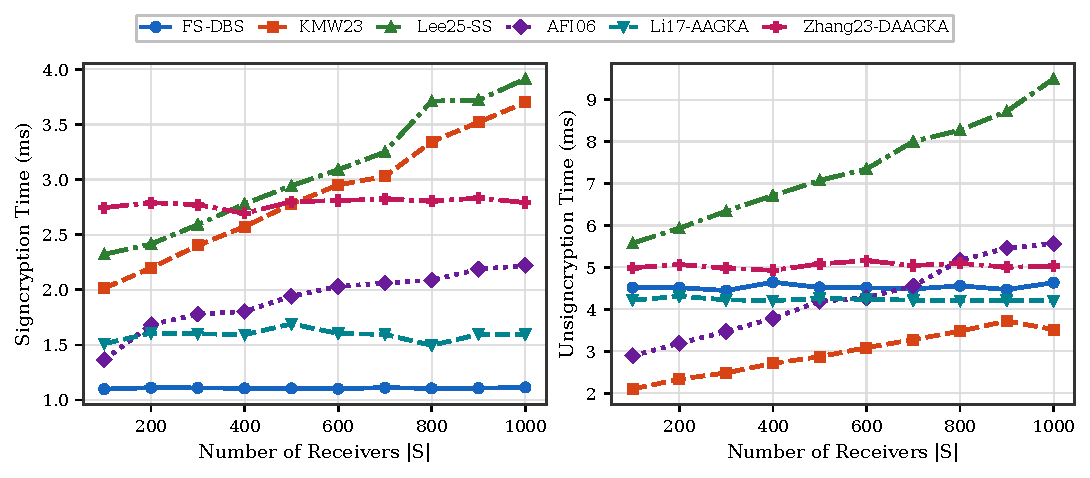
\includegraphics[width=0.92\textwidth]{figures/figure34_online_time.pdf}
	\caption{ Signcrypt and Unsigncrypt latency. The left panel reports
		the sender cost, and the right panel reports the receiver cost.}
	\label{fig:online-time}
\end{figure*}
\begin{table}[htbp]
	\caption{Experimental environment and benchmark parameters.}
	\label{tab:experimental-environment}
	\centering
	\small
	\setlength{\tabcolsep}{4.5pt}
	\renewcommand{\arraystretch}{1.10}
	\begin{tabular}{@{}p{0.38\columnwidth}p{0.56\columnwidth}@{}}
		\toprule
		\textbf{Item} & \textbf{Setting} \\
		\midrule
		Operating system   & Windows, x86-64 \\
		Processor          & Intel Core i7-14700HX \\
		Memory             & 32\,GiB \\
		Rust / Arkworks    & v1.91.0 / v0.5.0 \\
		Pairing    & BLS12-381, asymmetric Type-3 \\
		FS-DBS parameters & $n=1{,}024$ user slots; $d=20$ \\
		Receiver-set sizes & 10, 50, 100, 200, 500, 1000 \\
		\bottomrule
	\end{tabular}
\end{table}

\subsection{Computation Overhead}
Figure~\ref{fig:online-time} reports the online sender and receiver costs as
the authorized receiver-set size $|S|$ increases.
The vertical axis gives the median wall-clock time. Each point contains 20
timed samples, and each sample averages ten complete online calls. Setup,
registration, group establishment, and the formula-level recipient and time
terms defined as offline values are excluded. Pairing preprocessing is not
used.



At $|S|=1{,}000$, FS-DBS completes Signcrypt in 1.11\,ms. KMW23, Lee25-SS,
AFI06, Li17-AAGKA, and Zhang23-DAAGKA require 3.70, 3.91, 2.22, 1.59, and
2.79\,ms, respectively. FS-DBS therefore reduces the online sender latency by
69.9\%, 71.5\%, 49.8\%, 30.2\%, and 60.1\%, respectively. Its timed sender
path uses cached recipient-set and time-node terms and does not traverse the
receiver set. In contrast, the online encryption paths of KMW23, AFI06, and
Lee25-SS retain receiver-dependent group additions. Li17-AAGKA and
Zhang23-DAAGKA also have constant online paths after group establishment, but
execute their fixed Sign/Encrypt operations at each release.

FS-DBS requires 4.63\,ms for Unsigncrypt at $|S|=1{,}000$. Zhang23-DAAGKA,
AFI06, and Lee25-SS require 5.03, 5.56, and 9.50\,ms, so FS-DBS reduces their
receiver latency by 7.9\%, 16.7\%, and 51.2\%, respectively. KMW23 and
Li17-AAGKA require 3.51 and 4.20\,ms. These values are 24.2\% and 9.4\% below
FS-DBS, corresponding to absolute differences of 1.12 and 0.43\,ms. KMW23
evaluates two online pairing terms and does not provide integrated sender
authentication or time-key evolution. Li17-AAGKA evaluates four pairing terms,
whereas FS-DBS evaluates five terms to remove the broadcast and time masks and
to verify the sender. Lee25-SS incurs the largest receiver cost because its
decapsulation includes ciphertext validity checks and randomization.

\subsection{Epoch-Transition Overhead}
Figure~\ref{fig:epoch-transition} reports the time required to prepare one
receiver for the next epoch. The horizontal axis is the authorized group size,
and the vertical axis is the median wall-clock time. Each point contains 20
samples after five warm-up executions. FS-DBS and AFI06 execute one receiver
\textbf{KeyUpdate}. KMW23 and Lee25-SS generate one fresh receiver public/private
key pair. This operation is an operational reset baseline and does not add
forward security to either source DBE scheme. Li17-AAGKA and Zhang23-DAAGKA
execute a complete Agreement and encryption-key generation, followed by the
selected receiver's decryption-key generation.

At $n=1{,}000$, FS-DBS requires 13.20\,ms. AFI06, KMW23, Lee25-SS,
Li17-AAGKA, and Zhang23-DAAGKA require 19.23, 98.65, 97.44, 692.04, and
123.24\,ms, respectively. FS-DBS reduces the receiver transition latency by
31.3\%--98.1\% across these comparisons. The FS-DBS and AFI06 curves are
independent of $n$ because their updates operate on one time-tree state.
KMW23 and Lee25-SS are also independent of $n$ because the maximum user space
is fixed at 1,024 slots. The two AAGKA curves increase with $n$ because each
new group context aggregates all participant contributions. No pairing
preprocessing is used in this experiment.

\begin{figure}[htbp]
	\centering
	\Description{Broken-axis plot of median receiver epoch-transition latency for FS-DBS, AFI06, KMW23, Lee25-SS, Li17-AAGKA, and Zhang23-DAAGKA over authorized group sizes from 100 to 1,000.}
	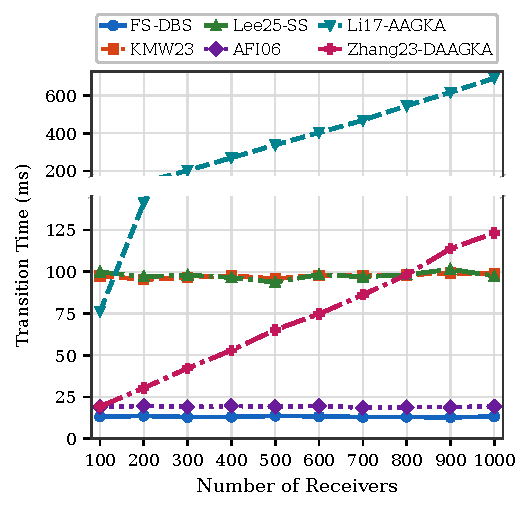
\includegraphics[width=\columnwidth]{figures/figure3_epoch_transition_time.pdf}
	\caption{Receiver epoch-transition latency. }
	\label{fig:epoch-transition}
\end{figure}

\subsection{Encrypted Model Distribution}
The model-distribution experiment uses the official TorchVision ResNet-50
IMAGENET1K\_V2 state dictionary, whose serialized size is 102,540,417 bytes.
The Advanced Encryption Standard with a 256-bit key in Galois/Counter Mode
(AES-256-GCM)~\cite{NISTSP80038D} encrypts the model body, and each public-key scheme protects only
the 32-byte content key. Ed25519 is added to schemes without integrated sender
authentication. Median AES encryption and decryption times are 46.01 and
45.40\,ms. Median Ed25519 signing and verification times are 0.013 and
0.023\,ms.

Figure~\ref{fig:model-update} considers 100 authorized receivers and 100 model
releases. A state transition, fresh-key reset, or group re-agreement is invoked
after every ten completed releases. The horizontal axis is the number of model
releases, and the vertical axis is cumulative security-layer time. Panel (a)
contains one sender operation, one receiver operation, and the corresponding
epoch path. Panel (b) reports the aggregate work for the sender and all 100
receivers as sequential single-core-equivalent computation. The common
AES-256-GCM and network-transfer costs are excluded from both panels.

At 100 releases in panel (a), FS-DBS requires 0.580\,s. Zhang23-DAAGKA, AFI06,
Li17-AAGKA, KMW23, and Lee25-SS require 0.658, 0.964, 1.121, 1.845, and
2.514\,s, respectively. FS-DBS reduces these costs by 11.8\%, 39.8\%, 48.2\%,
68.5\%, and 76.9\%. The result follows from the fixed online sender and receiver
paths and the noninteractive KeyUpdate operation. Li17-AAGKA and
Zhang23-DAAGKA execute a complete Agreement and key-generation path at each
epoch boundary. KMW23 and Lee25-SS use fresh key pairs only as an operational
reset baseline; this reset does not add forward security to the source schemes.

At the same endpoint in panel (b), FS-DBS requires 40.72\,s of aggregate work.
AFI06, KMW23, and Lee25-SS require 71.10, 146.50, and 209.52\,s. FS-DBS is
42.7\%, 72.2\%, and 80.6\% below these values, respectively.
Li17-AAGKA and Zhang23-DAAGKA require 32.74 and 34.56\,s. These values are
19.6\% and 15.1\% below FS-DBS, with absolute differences of 7.99 and 6.16\,s
over the full sequence. Their lower aggregate CPU totals arise because an
established group context avoids updating 100 independent time-tree states.
Their epoch transitions instead require group agreement and synchronization.
Panel (b) excludes this communication delay and should not be interpreted as
network wall-clock latency.

\begin{figure}[htbp]
	\centering
	\Description{Cumulative public-key security-layer time versus the number of periodic model releases.}
	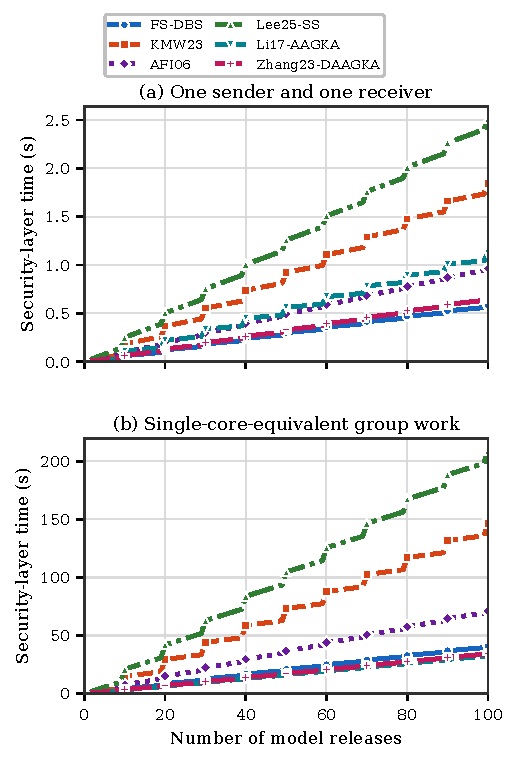
\includegraphics[width=\columnwidth]{figures/figure6_model_update.pdf}
	\caption{Cumulative security-layer time for periodic model releases.}
	\label{fig:model-update}
\end{figure}
\section{Conclusion}
This paper presented FS-DBS for authenticated cloud-to-edge data distribution.
It provides constant-size ciphertexts, and its online computation is independent
of the receiver-set size. We prove selective FS-IND-CCA confidentiality and
selective EUF-CMA unforgeability in the random oracle model under the dBDHE
assumption.

Our implementation over BLS12-381 shows that FS-DBS maintains low online and key-update costs as the receiver set grows. At 1,000 receivers, signcrypt, unsigncrypt, and key update require 1.11 ms, 4.63 ms, and 13.20 ms, respectively. In the ResNet-50 distribution experiment, FS-DBS also reduces latency for repeated cloud-to-edge delivery. These properties make FS-DBS suitable for distribution scenarios that require both protection against receiver-key exposure and low per-release overhead.

Future work will consider adaptive security and constructions that avoid reliance on the random oracle model. Another direction is to strengthen the system model against imperfect key erasure and rollback of receiver states. We also plan to evaluate FS-DBS on heterogeneous edge devices and wide-area deployments to study computation, state-update, and network costs under practical deployment conditions.
\bibliographystyle{ACM-Reference-Format}
\bibliography{Ref}
\end{document}
\endinput
%%
%% End of file `sigconf.tex'.
